\documentclass[../main.tex]{subfiles}
\graphicspath{{\subfix{../IMAGES/}}}

\begin{document}
\localtableofcontents

\subsection{Modélisation d'une turbine Pelton à l'aide d'une machine à courant continu}


Caractérisation de la machine à courant continu : \\
\begin{itemize}
    \item mesure de la résistance de l'induit : le courant circulant dans la MCC passe par des charbons (commutateur) afin de passer dans les bobines du rotor et sort de la MCC en repassant par les charbons. Pour mesurer la résistance $R_{ind}$, il est donc préférable d'utiliser un générateur de courant et de mesurer la chute de tension. Un ohmmètre quant à lui n'envoie que quelques $mA$, ce qui est nettement inférieur au courant nominal et peut donc fausser la mesure. \\
    Envoi de 4.94A, chute de tension de 16V soit $\mathbf{R_{ind} = 3.23\Omega}$.\\
    \item mesure du facteur $k_{\phi, MCC}$ : utilisation d'une machine asynchrone afin de faire tourner l'arbre de la MCC à 1500t/min et mesure de la tension au borne de la MCC
    \begin{figure}[hbt!]
        \centering
        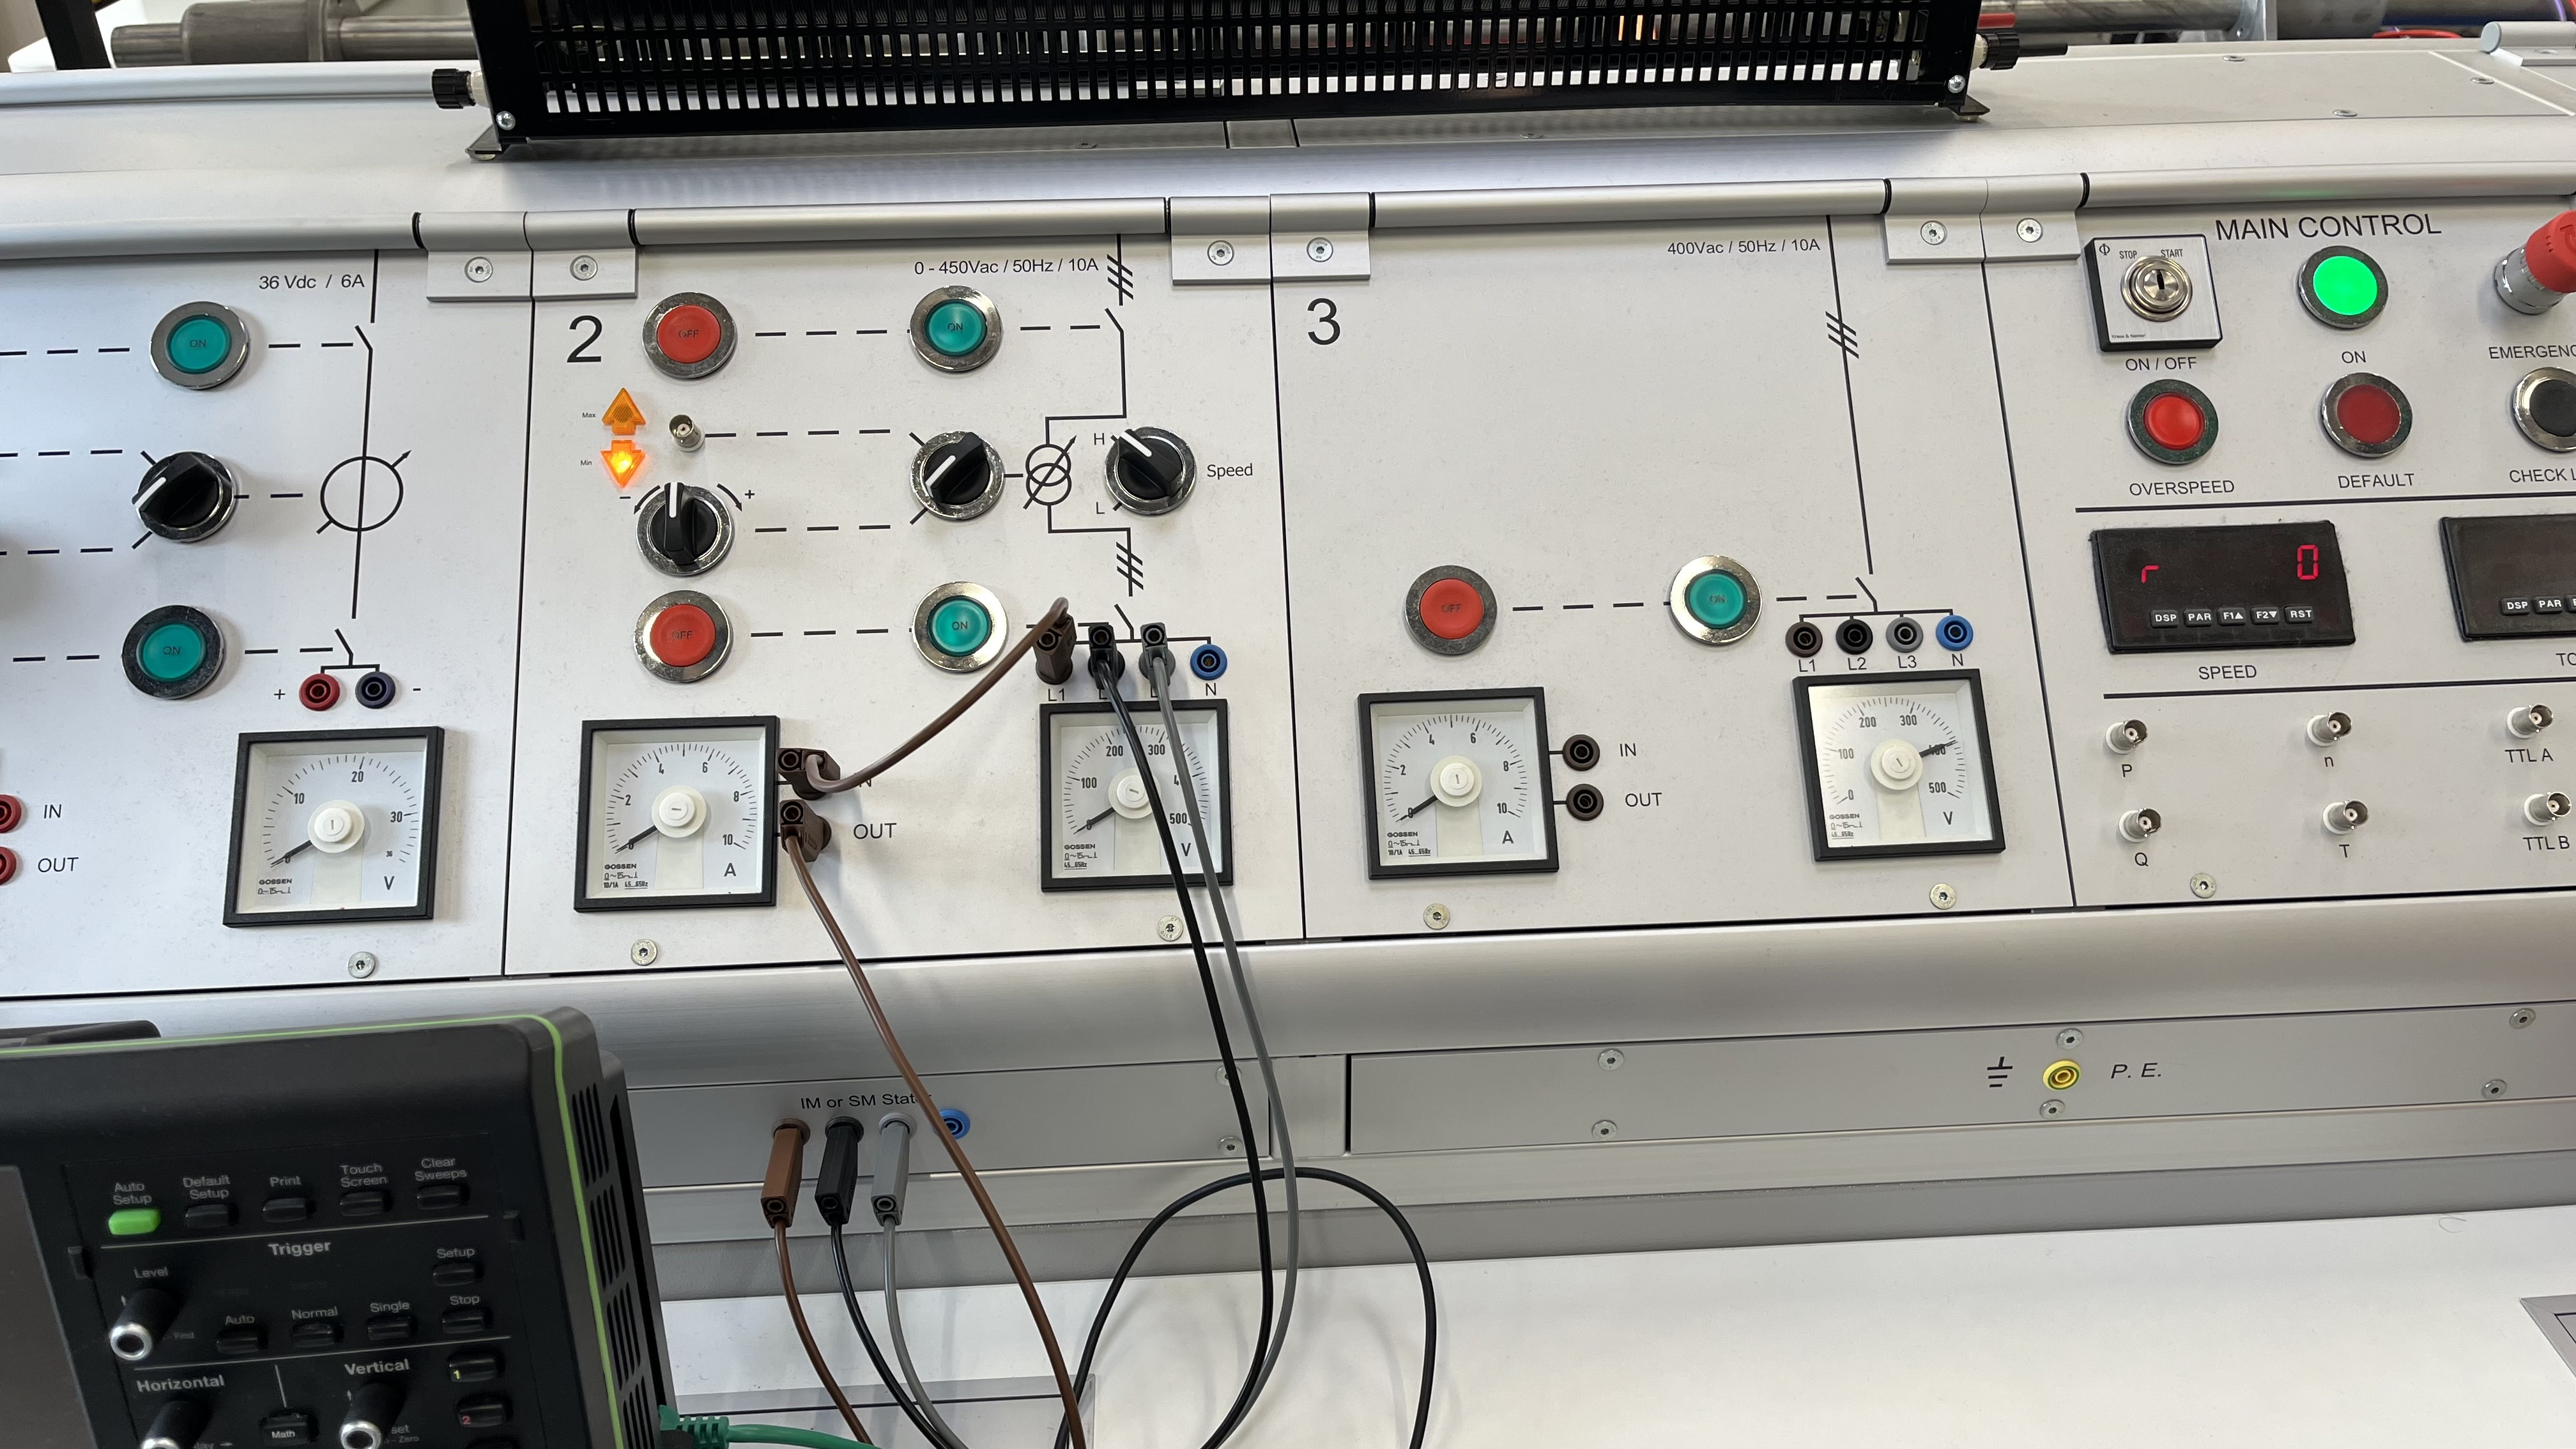
\includegraphics[width=0.5\linewidth]{IMAGES/ALEEL/IMG_2164.jpg}
    \end{figure}
    \begin{figure}[hbt!]
        \centering
        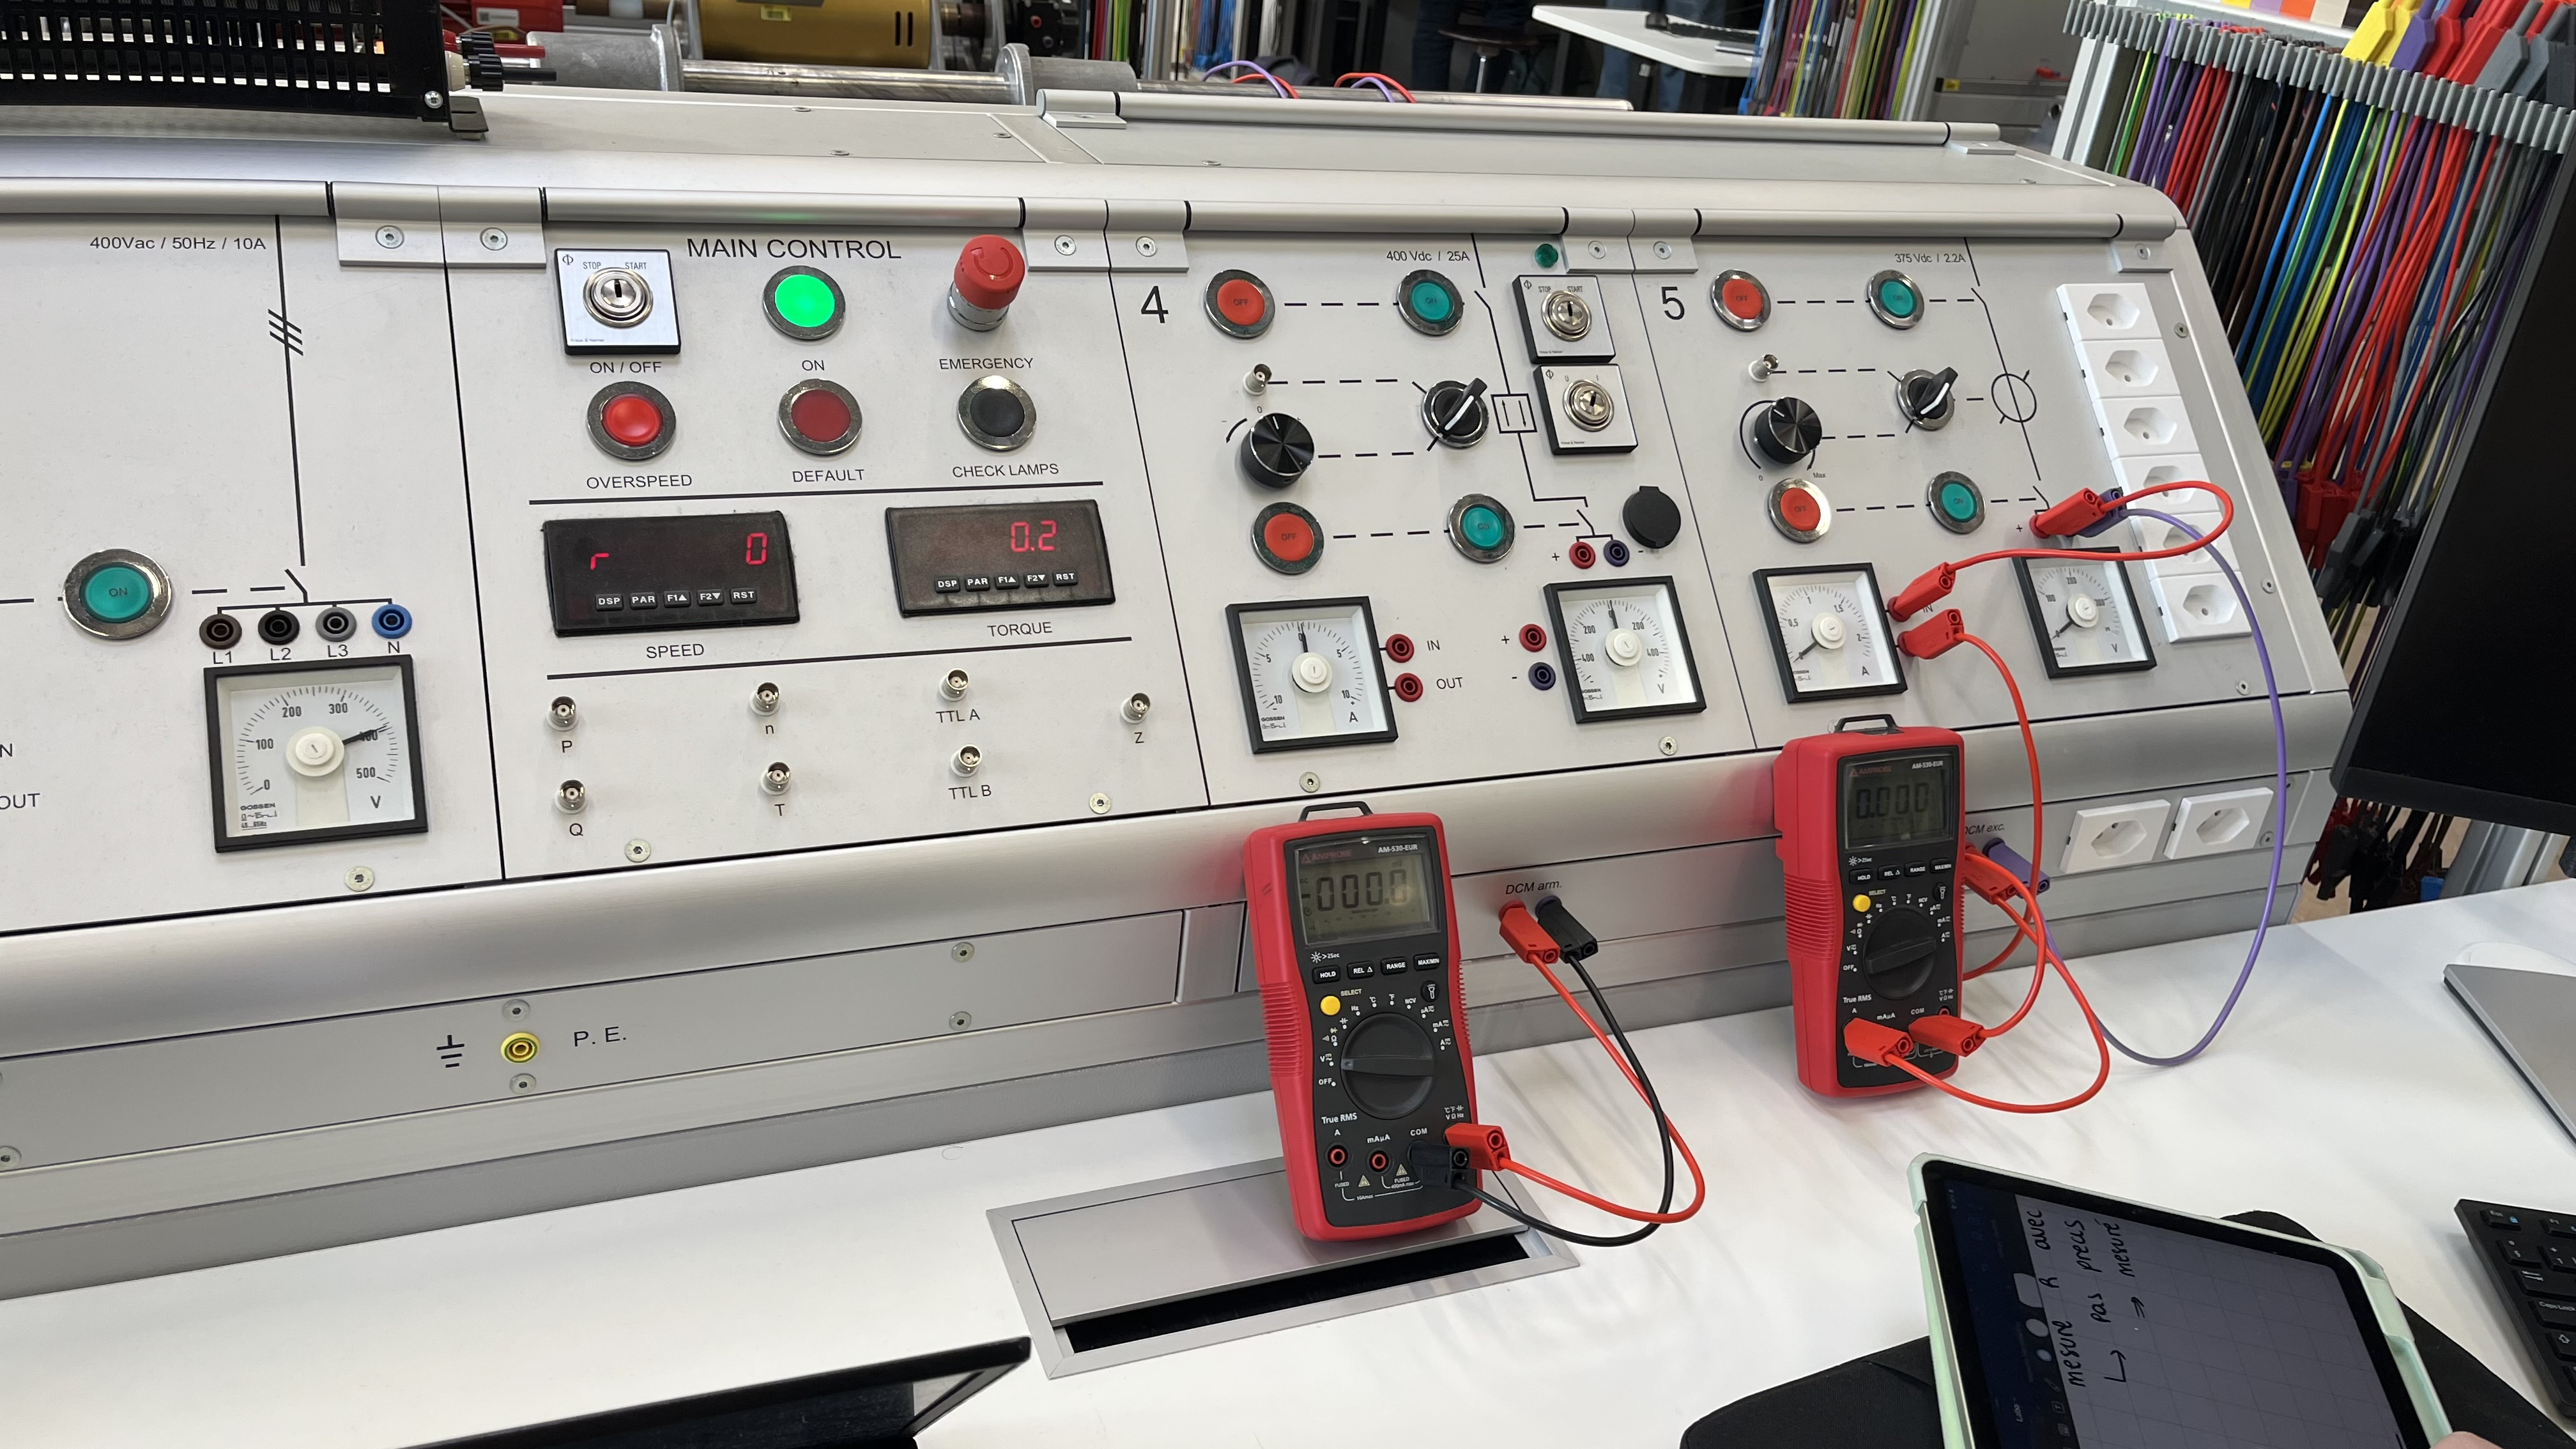
\includegraphics[width=0.5\linewidth]{IMAGES/ALEEL/IMG_2165.jpg}
    \end{figure}
    $\mathbf{k_{\phi, MCC}} = \frac{U_i}{\Omega} \mathbf{= 1.69\pm 0.195\%}$\\
    \item Calcul de $U_{MCC}$ et $R_{add}$ : caractéristique de couple de la MCC : $T_{em} = k_{\phi, MCC}  \frac{U_{MCC} - k_{\phi, MCC} \omega}{R}$. Lors $\omega = \omega_0 \Rightarrow T_{em} = 0Nm$, lorsque $\omega= \omega_n \Rightarrow T_{em} = T_n$. \begin{equation}
        \begin{gathered}
            U_{MCC} = k_{\phi, MCC} N_0 \frac{2\pi}{60} = 354.34V\\
            R_{add} = \frac{k_{\phi, MCC} U_{MCC} }{T_{max}}-R_{ind} = 26.73\Omega\\
        \end{gathered}
    \end{equation}
    \warning A noter que la résistance additionnel vient en série avec la MCC afin de lui donner la même caractéristique que la génétrice Pelton. \\
\end{itemize}

\begin{figure}[hbt!]
    \centering
    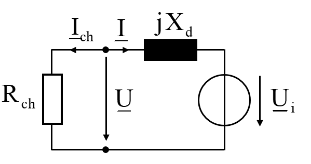
\includegraphics[width=0.4\linewidth]{IMAGES/ALEEL/Screenshot from 2025-02-27 21-36-40.png}
    \caption{Schéma équivalent machine synchrone avec charge}
\end{figure}

Soit $T_{mec} = 5Nm$ le couple mécanique de l'arbre, $U = U_n = 230V$, $50Hz$, $x_d = 1.5 p.u.$ et $P_0 = 200W$ les pertes fer/ventilation.\\
La résistance interne à la MS (machine synchrone) est négligeable. Dès lors, la puissance électrique en sortie de la machine vaut : $P_{el} = T_{mec} \omega - P_0 = 585.39W = 3UI$ (charge purement résistive). La résistance de charge vaut donc : $\mathbf{R_{ch} = 3\frac{U^2}{P_{el}} = 271\Omega}$ et le courant de charge : $\mathbf{I_{ch}} = -I = \frac{U}{R_{ch}} \mathbf{= 0.84A}$.\\
La tension induite (de par le schéma équivalent) vaut maintenant : $\underline{U}_i = Z_{tot} \underline{I} = (R_{ch} + iX_d) \underline{I}$. Or : $X_d = x_d Z_{base} = x_d 3 \frac{U^2}{S_{base}} = 99.18\Omega$. Ainsi, $\mathbf{U_i = 244.9V}$. Le facteur $\mathbf{k_{\phi,MS} =} \frac{U_i}{\omega} = \mathbf{1.56} \frac{V}{rad/s}$. L'angle $\delta$ de déphasage est calculé via : $P_{el} = \frac{UU_i}{X_d}\sin\delta$, soit : $\mathbf{\delta = 0.35rad = 20.1^\circ}$.\\

Lors du changement de charge ($R_{ch}' = 1.1R_{ch}$), la puissance électrique, vitesse, tension, courant, angle de déphasage, $\cdots$ changent. On repart donc de l'équation caractéristique de couple de la MCC : $T_{mec} = k_{\phi,MCC} \frac{U_{MCC}-k_{\phi,MCC}\omega}{R}$. Du côté de la MS : $P_{el} = 3 R_{ch}' I^2 = P_{mec}-P_0 = \omega T_{mec} - P_0$. De plus : $U_i = k_{\phi,MS} \omega$ et $I = \frac{U_i}{\lvert Z_{tot}'\rvert}$ avec $Z_{tot}' = R_{ch}' + iX_d$. En rassemblant tous les termes, on trouve : \begin{equation}
    (3 \frac{R_{ch}' k_{\phi, MS}^2}{\lvert Z_{tot} \rvert^2} + \frac{k_{DC}^2}{R}) \omega^2 - \frac{k_{DC} U_{MCC}}{R} \omega + P_0 = 0
\end{equation}
Deux solutions à cette équation, une faisable une non faisable(vitesse de rotation trop faible). On obtient donc : $N = 1523.36RPM$, soit $\mathbf{n = 25.38t/s}$. \\
Le courant est dès lors : $\mathbf{I' =} k_{\phi, MS} \frac{\omega}{\lvert Z_{tot} \rvert} = \mathbf{0.7914A}$. Le voltage quant à lui : $\mathbf{U'} = R_{ch}' I' = \mathbf{236.01V}$. \\
L'angle de déphasage est ainsi : $\mathbf{\delta =} \arcsin(\frac{P_{el} X_d}{3 U U_i}) = \mathbf{0.3211rad = 18.39^\circ}$.\\

\quad \underline{Vérification pratique :}\\
Afin de vérifier nos résultats théoriques, nous avons effectué une mise en pratique du système. Tout d'abord une vérification des $k_\phi$ des deux machines (MS et MCC). \begin{itemize}
    \item Machine MCC : utilisation de l'équation $U = R_{ind} I + U_i$, en faisant varier le voltage (avec une excitation de 0.2A), on peut mesurer le courant ainsi que la vitesse de rotation de l'arbre pour obtenir : $k_{\phi, MCC} = \frac{U-R_{ind} I}{\omega}$. Par cette méthode, on obtient : $k_{\phi, MCC} = 1.64\pm 0.34 \frac{V}{rad/s}\%$, soit une différence de $-3\%$ par rapport à la mesure précédente.
    \item Machine MS : avant de mesurer le $k_\phi $ de la MS, il faut trouver le $I_{f0}$ (courant d'excitation à vide). Pour ce faire, il faut faire tourner la MS à 1500t/min et augmenter $I_f$ jusqu'à ce que $V_{phase} = 230V$. On obtient dès lors : $\mathbf{I_{f0} = 2.28A}$. Pour mesurer le $k_\phi$ de la MS on mesure la tension de phase de la machine (qui correspond à $U_i$ lorsque la charge est nulle) lorsque la vitesse de rotation de l'arbre change (en utilisant la MCC) : $k_{\phi, MS} = \frac{U_i}{\Omega}$. On obtient dès lors $\mathbf{k_{\phi, MS} = 1.46 \pm 0.36\%} \frac{V}{rad/s}$, soit une différence de $-6.4\%$ par rapport à la valeur calculée.
\end{itemize}

\quad \underline{Vérification charactéristique couple/vitesse :}\\

Pour vérifier la charactéristique de couple/vitesse de la MCC, il faut brancher en série la résistance $R_{add} = 26.73\Omega$ à l'armature de la MCC ainsi que la résistance de charge à la MS : $R_{load} = 271\Omega$.\\
La MCC est excitée avec un courant de $I_f = 0.2A$(vérifié avec un ampèremètre) et alimentée avec tension de $U_{MCC} = 354V$ (vérifiée avec un voltmètre). La MS est quant à elle excitée avec un courant $I_{f0} = 2.28A$ (vérifié avec un ampèremètre) et une charge branchée en étoile. \warning La tension de phase est vérifiée avec un voltmètre pour ne pas dépasser $265V$! Le couple résistif sur l'arbre est changé via un changement de la charge. La charge est donc changée de manière continue afin de passer de 0 à $1.5 T_n$ (soit $7.5Nm$).\\
\begin{figure}[hbt!]
    \centering
    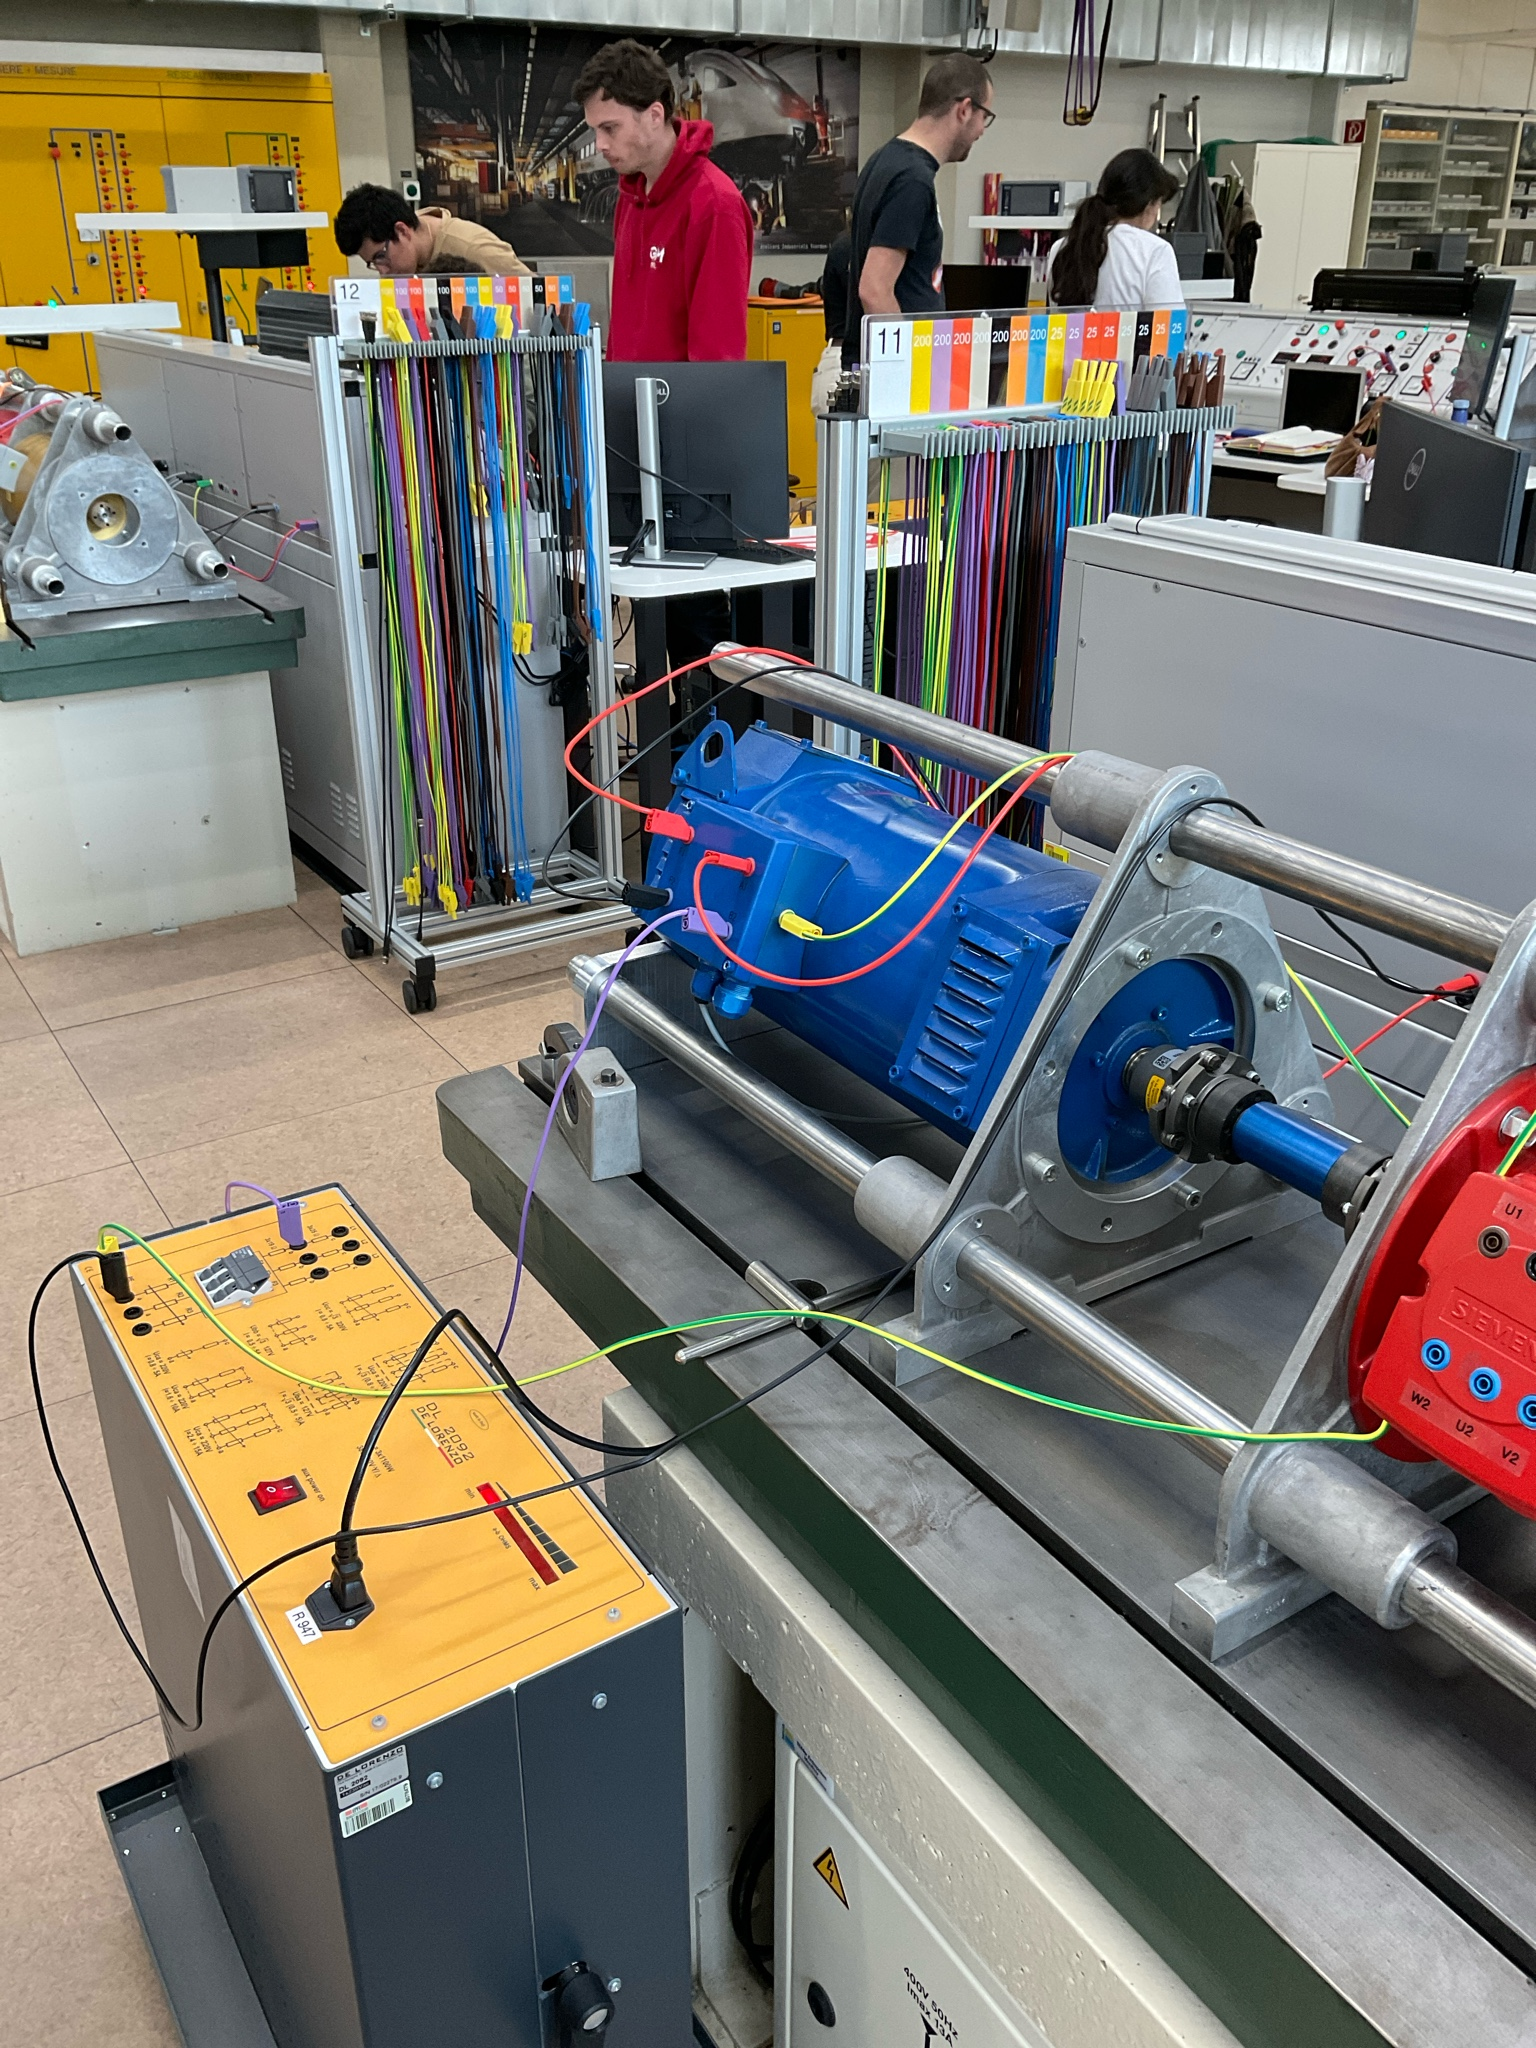
\includegraphics[width=0.6\linewidth]{IMAGES/ALEEL/Image 08.03.2025 at 19.38 (2).jpg}
    \caption{$R_{add}$}
\end{figure}
\begin{figure}[hbt!]
    \centering
    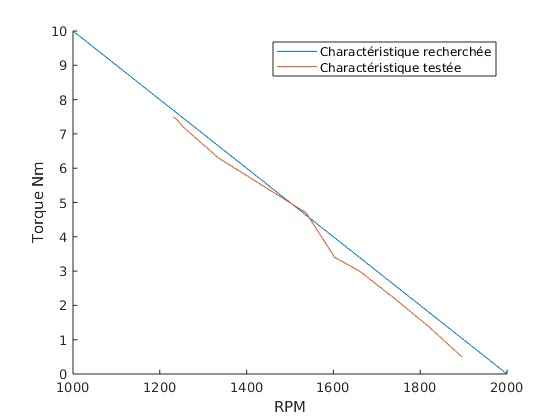
\includegraphics[width=0.7\linewidth]{IMAGES/ALEEL/verif_charac.jpg}
\end{figure}

La charactéristique mesurée est identique à celle désirée! La différence maximale relative à la charactéristique idéale est de : $-4\%$ avec un RMSE de $0.37Nm$.\\

\quad \underline{Vérification de la charge, angle de déphasage, tension :}\\
Lorsque la charge vaut $271\Omega$ par phase branchée en étoile à la MS avec une excitation de $I_{f0} = 2.28A$, on obtient bien une vitesse de rotation de $1500t/min$, une tension de phase de $230V$.

\begin{figure}[hbt!]
    \centering
    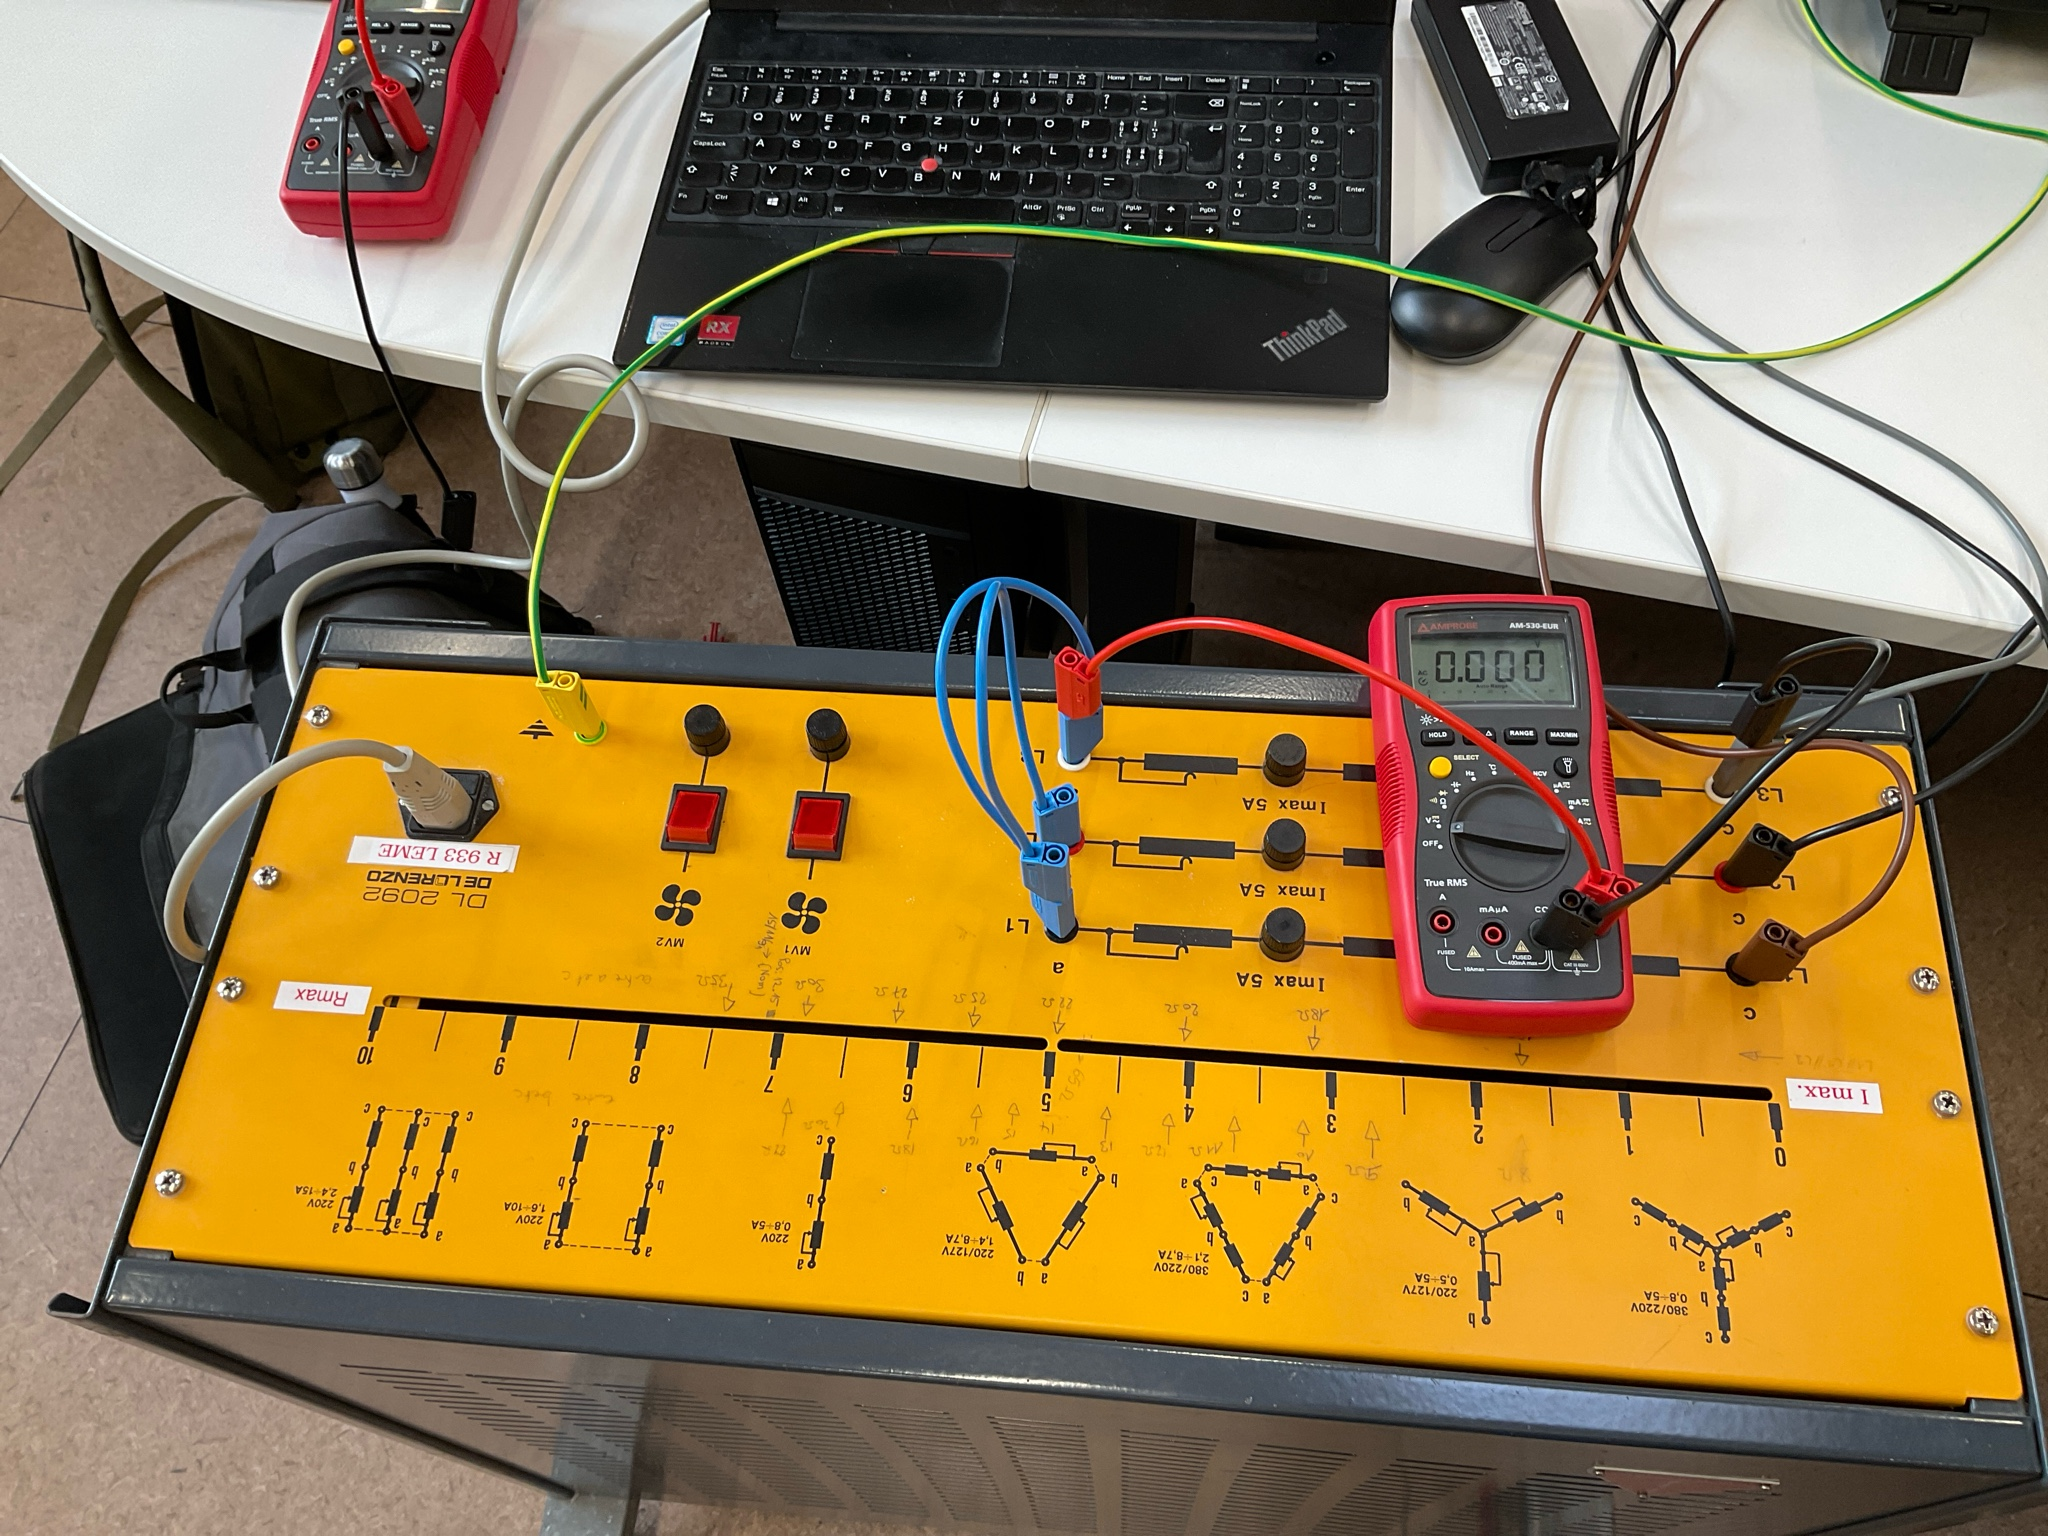
\includegraphics[width=0.6\linewidth]{IMAGES/ALEEL/Image 08.03.2025 at 19.38 (1).jpg}
    \caption{$R_{load}$}
\end{figure}

De plus, $U_i = k_{\phi, MS} \omega = 229.19V$ et $I = 0.846A$, soit $P_{el} = 583.74W$. Dès lors, on a $\delta = \arcsin(\frac{P_{el} X_d}{3UU_i}) = 0.374 rad = 21.48^\circ$ soit une erreur de $6.8\%$ par rapport à la valeur calculée.\\

\quad \underline{Saut de tension :}\\

\begin{figure}[hbt!]
    \centering
    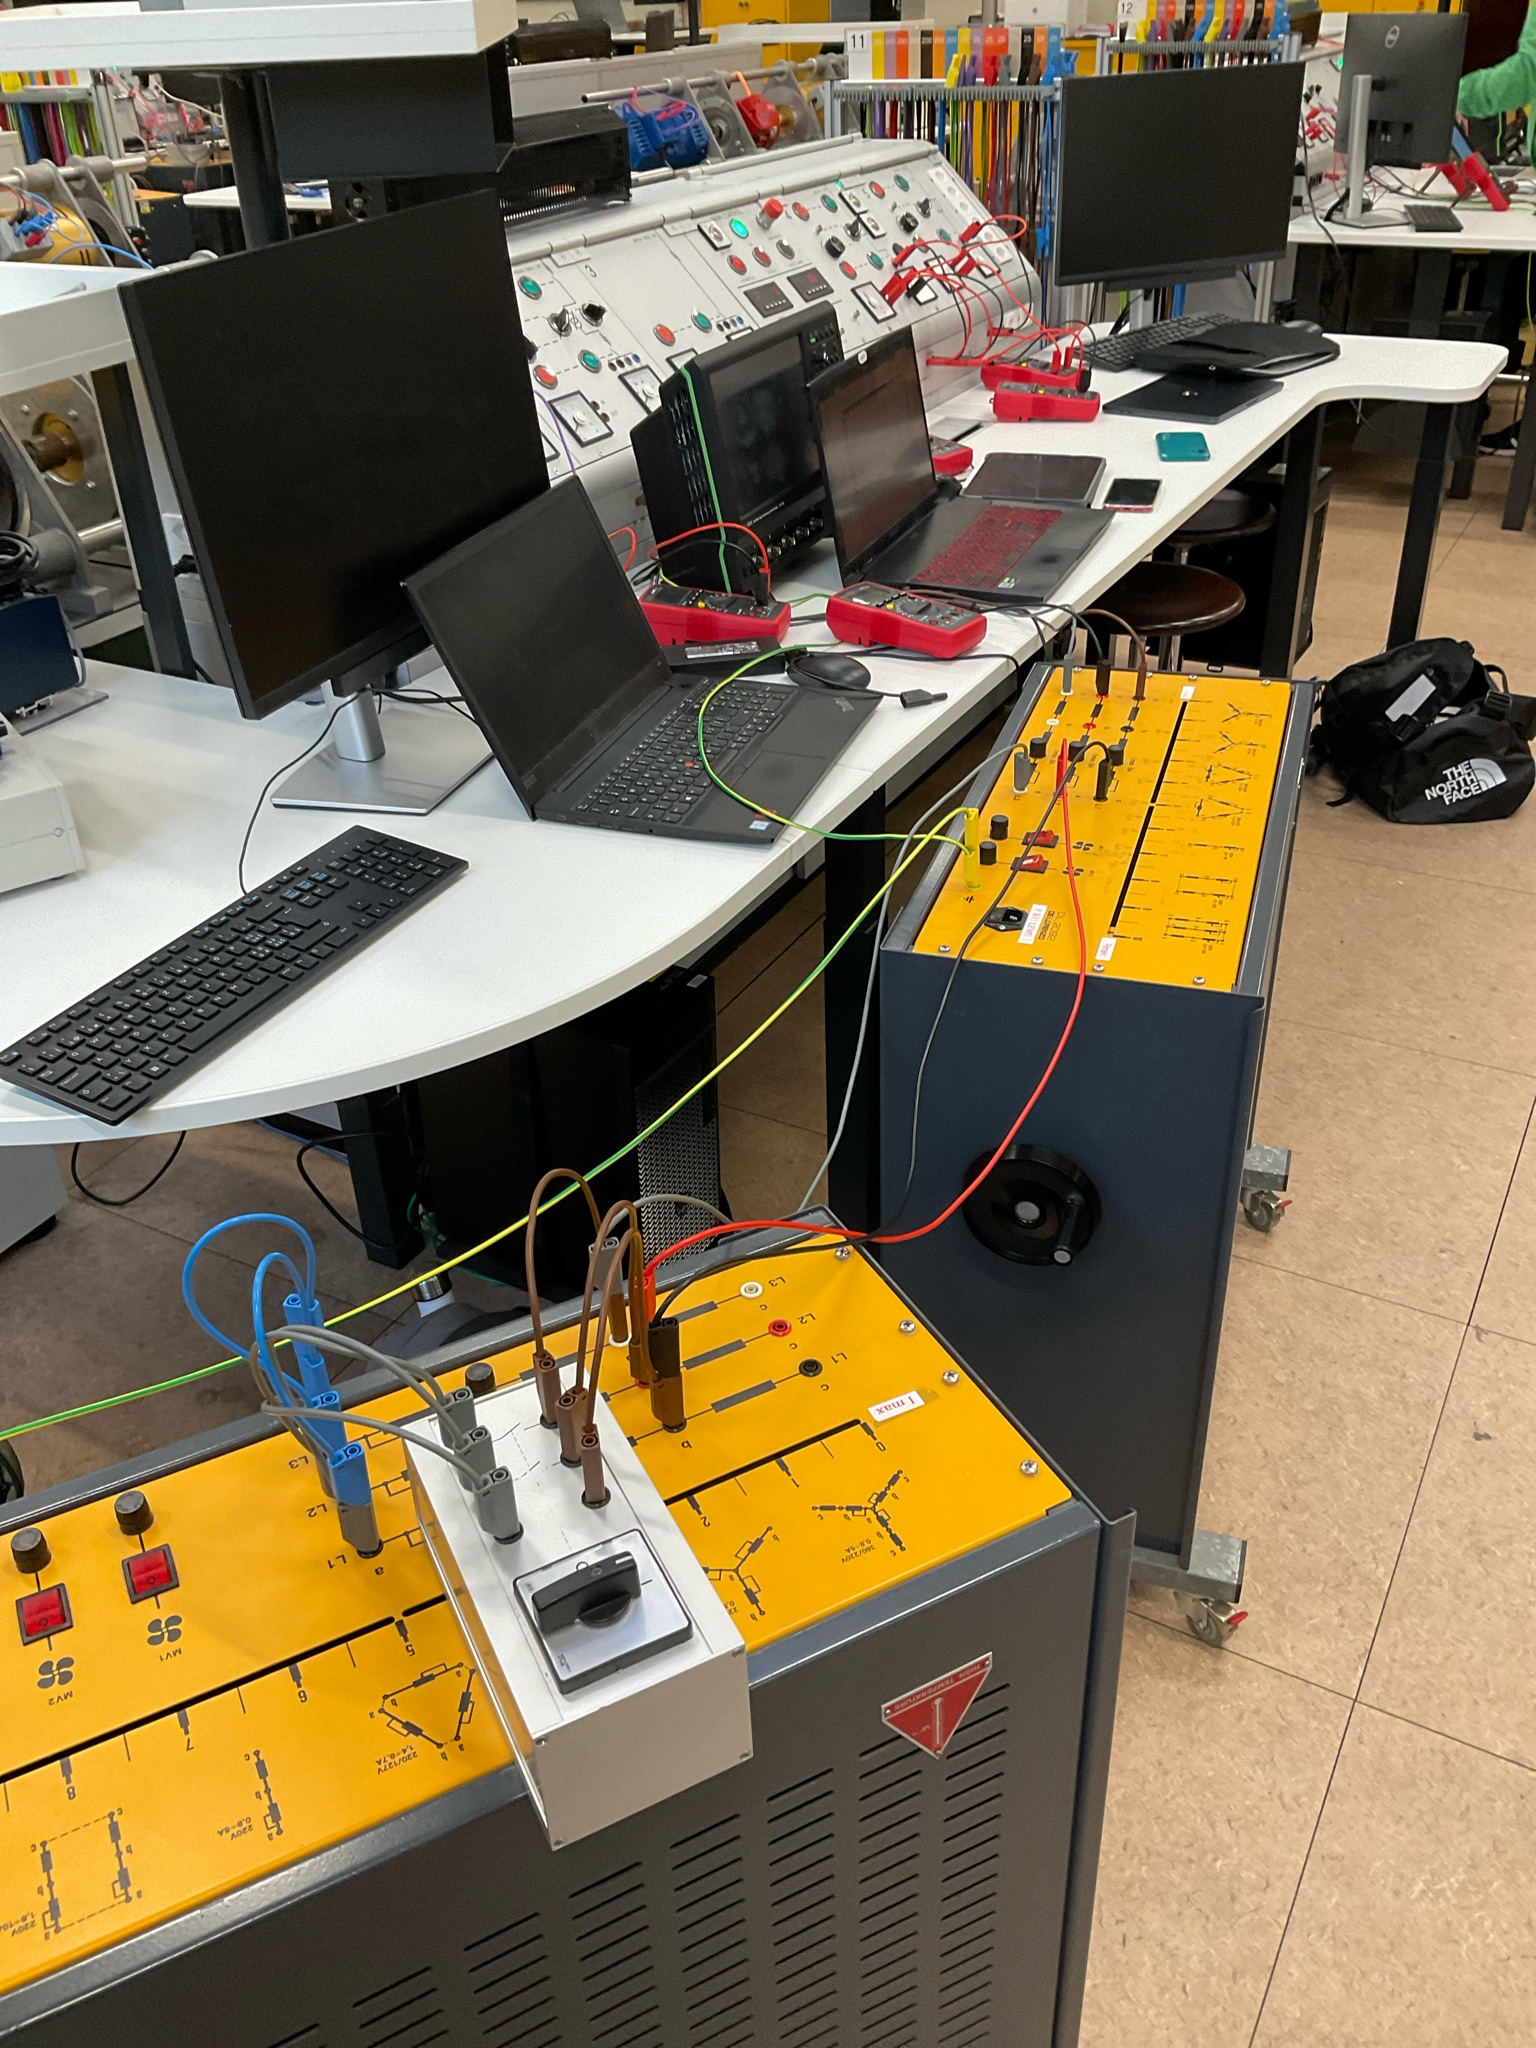
\includegraphics[width=0.6\linewidth]{IMAGES/ALEEL/Image 08.03.2025 at 19.39 (1).jpg}
    \caption{Ajout d'une résistance en série pour obtenir $R_{ch}'$.}
\end{figure}
Le saut de tension est réalisé en ajoutant en série une résistance de $27.1\Omega$ par phase. Lorsque le système est stabilisé pour $R_{ch}$ les valeurs sont récupérées puis le saut de tension est effectué pour passer à $R_{ch}'$ et lorsque le système est stabilisé les valeurs sont récupérées.\\

\begin{table}[hbt!]
    \centering
    \begin{tabular}{c|c|c|c|c}
        Variable & Valeur pour $R_{ch}$ & Valeur pour $R_{ch}'$  & Valeur attendu après le saut de charge & Erreur relative\\ \hline
        $I$ & $0.846A$ & $0.781A$ & $0.791$ & $-1.3\%$\\
        $U$ & $230V$ & $234V$ & $236V$ & $-0.8\%$\\
        $n$ & $1544 t/min$ & $1564t/min$ & $1523t/min$ & $2.66\%$\\
        $T$ & $4.4Nm$ & $4.2Nm$ & $4.76Nm$ & $-11\%$\\
    \end{tabular}
    \caption{Variation lors du saut de charge}
\end{table}

\quad \underline{Modélisation Simscape :}\\

\begin{figure}[hbt!]
    \centering
    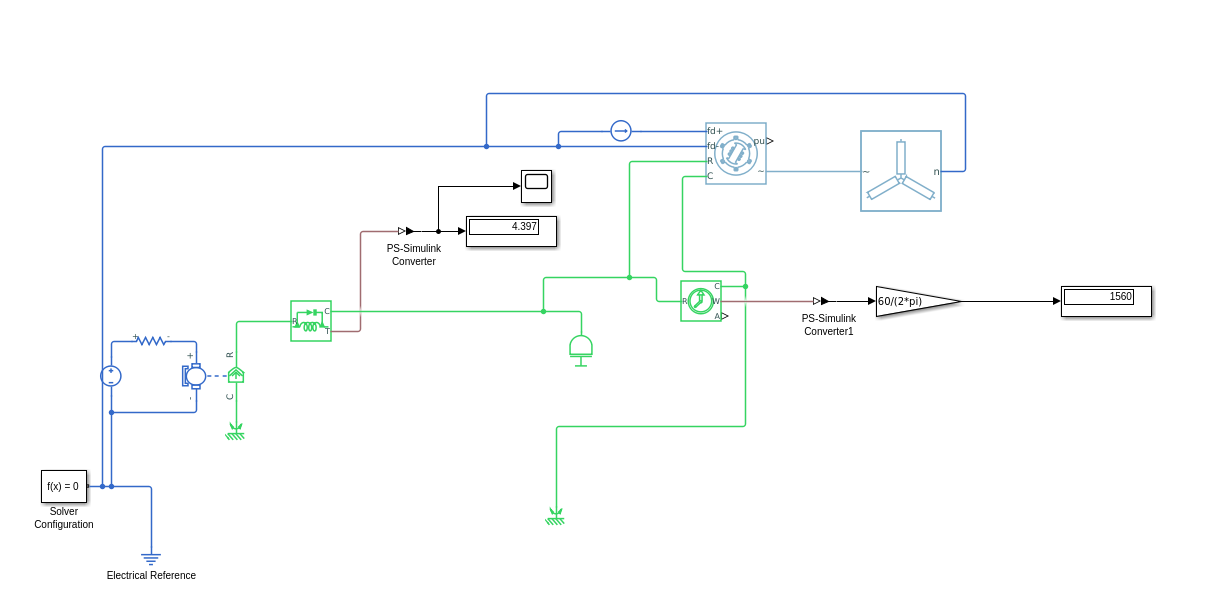
\includegraphics[width=\linewidth]{IMAGES/ALEEL/Screenshot from 2025-03-13 14-57-59.png}
    \caption{Simscape}
\end{figure}

\begin{figure}[hbt!]
    \centering
    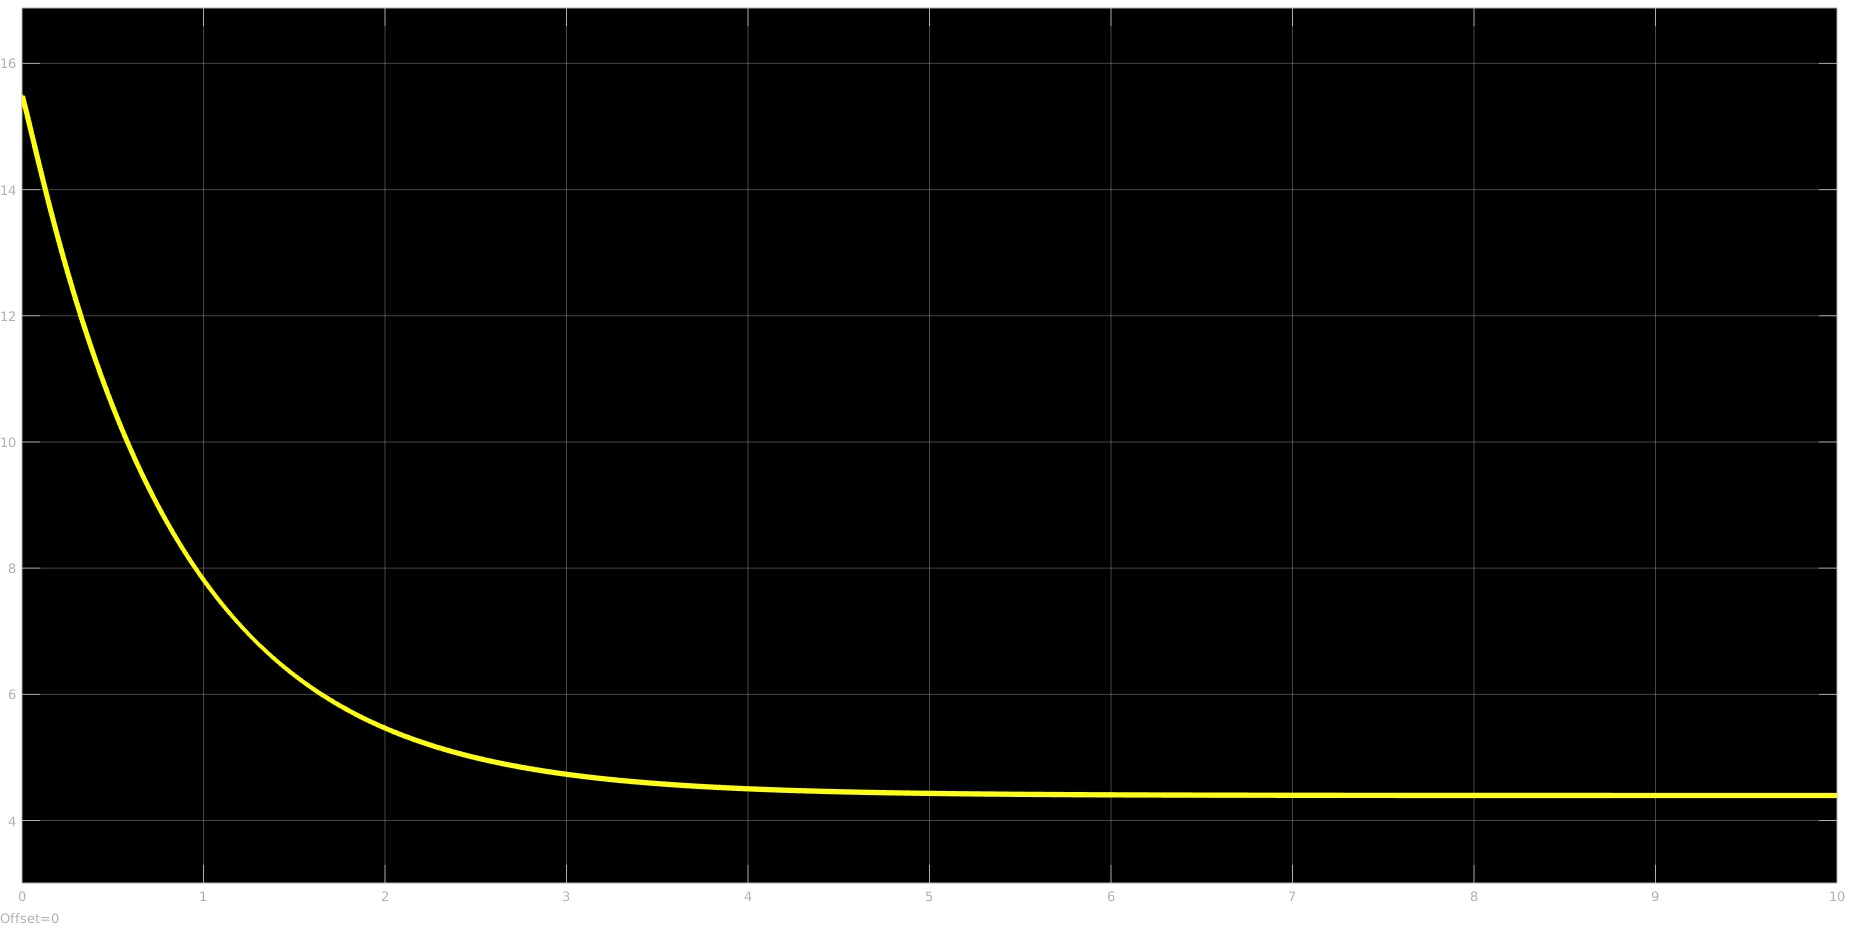
\includegraphics[width=\linewidth]{IMAGES/ALEEL/Torque_simulink.jpg}
    \caption{Couple vs. temps}
\end{figure}

\subsection{Réglage vitesse MCC}



\begin{figure}[hbt!]
    \centering
    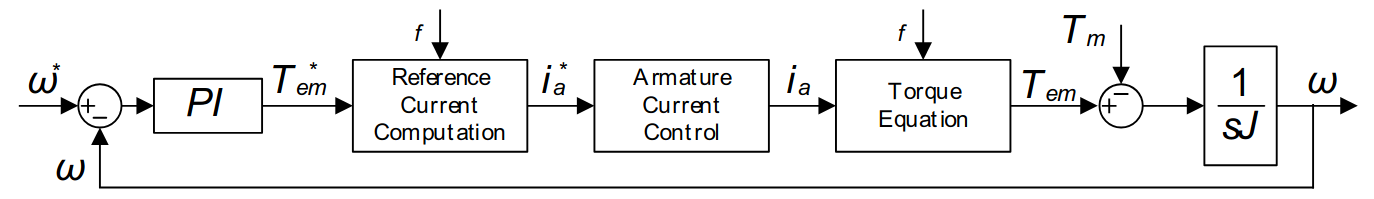
\includegraphics[width=0.5\linewidth]{IMAGES/ALEEL/Screenshot from 2025-03-31 11-11-00.png}
    \caption{Schéma de contrôle en vitesse de la MCC}
    \label{fig:schemaMCCspeed}
\end{figure}

Le contrôle en vitesse de la MCC se fait à l'aide de deux contrôleur PI; un contrôleur de courant dans l'armature qui forme la boucle interne et un contrôleur de vitesse qui forme la boucle externe comme indiqué sur \ref{fig:schemaMCCspeed}.\\
Dans notre cas, le contrôleur de courant est intégré au banc de test; nous devons donc approximer son effet. Pour ce faire, nous supposons qu'il s'agit d'un délai de premier ordre:
\begin{equation}
    G_{cl,a}(s) = \frac{1}{1+sT_{pE}}\hspace{20pt}\text{avec}\hspace{20pt} T_{pE} = \frac{T_E}{2}+ T_{ea} + T_r
\end{equation}
$T_{pE}$ représente la somme de tous les délais présents dans la boucle fermée du contrôleur de courant, qui doivent être évalués. Ces délais incluent le temps d'échantillonnage $T_E = 1ms$, le temps nécessaire pour que le signal atteigne un état stable $T_{ea}$, ainsi que le temps de réponse de la machine à courant continu face à une variation soudaine de la commande en courant $T_r$.\\
L'éxpression qui décrit le contrôle en vitesse est:$ \hspace{10pt} T_m\frac{dn}{dt} = i_a-m_r$\\
Ce modèle peut être exprimé sous la forme d'une fonction de transfert d'un intégrateur pur, soit: $ \hspace{10pt} P(s) = \frac{1}{T_m s}$. \\
Un contrôleur PI peut donc être utilisé pour régler la vitesse de la MCC avec un réglage utilisant le critère symétrique. Les coefficients du contrôleur PI $C(s) = \frac{1+sT_n}{sT_i}$ sont calculés comme suit: 
\begin{gather}
    T_n = 4 T_{pE} \hspace{30pt} T_i = 8 \frac{T_{pE}^2}{T_1} = 8 \frac{T_{pE}^2}{J}
\end{gather}
Nous souhaitons également appliquer un correcteur de consigne afin de limiter le dépassement de la réponse en vitesse de la MCC. Pour ce faire, on applique une fonction de transfert: 
\begin{equation}
    G_w(s) = \frac{1}{1+sT_{cw}}\hspace{20pt}\text{avec}\hspace{20pt}  T_{cw} = 4T_{pE}
\end{equation}
Après discrétisation, l'expression du correcteur devient: 
\begin{gather}
    n_{cw}[k+1] = K_{cw1}n_{cw}[k] + K_{cw2} n_c [k] \hspace{20pt}
    \text{avec}\hspace{20pt} K_{cw1} = e^{-\frac{T_E}{T_{cw}}}; K_{cw2} = 1-K_{cw1}
\end{gather}

\subsubsection{Algorithme de réglage}

\begin{verbatim}
function [regOutLim, integratorOut]  = 
  =fcn(speedSetValue, speedMeasure, regulationMode, Kp, Ki, Kwc1, Kwc2, LIMREG)
%% v02 : avec Théorique
%% constants definition
STANDARD    = 0;   % Standard mode (no ARW, no Cor)
GLOBAL      = 1;   % Global mode for the controller (ARW + Cor)
ARW         = 2;   % Anti-reset Windup mode (only ARW)
CORRECTOR   = 3;   % Corrector mode (only Cor)
THEORETICAL = 4;   % Theoretical mode (no ARW, no Cor, no Limitation)

% initialisation 
persistent wc
if isempty(wc)
    wc = 0;
end
persistent integrator
if isempty(integrator)
    integrator = 0;
end
%% correcteur de consigne
if (regulationMode == GLOBAL || regulationMode == CORRECTOR)
    CorrectSetPoint = wc;
    wc = Kwc1*wc+Kwc2*speedSetValue;
else
    CorrectSetPoint = speedSetValue;
end
%% Control
error = CorrectSetPoint-speedMeasure;
proportional = (Kp+Ki)*error;
%integrator = integrator+Ki*error;
regOut = proportional + integrator;
%% Integrator
if regulationMode ~= THEORETICAL && regulationMode ~= CORRECTOR
    if regOut>LIMREG
        regOutLim = LIMREG;
    elseif regOut<-LIMREG
        regOutLim = -LIMREG;
    else
        regOutLim = regOut;
    end
else
    regOutLim = regOut;
end
%%ARW
if (regulationMode == GLOBAL || regulationMode == ARW)
    error = error - 1/(Kp+Ki)*(regOut-regOutLim);
end
integrator = integrator + Ki*error;
%% DO NOT EDIT ------------------------------------------------------------
integratorOut = integrator; % Integrator Output for display
\end{verbatim}

\warning Ce code correspond aux simulations hors-ligne en simulink. Dans le cas des tests en conditions réelles sur le compact rio, la limitation est active pour tous les modes. 

\subsubsection{Mesure des constantes}

\begin{itemize}
    \item Conversion commande en voltage donnée/réponse du banc en courant : \begin{figure}[hbt!]
        \centering
        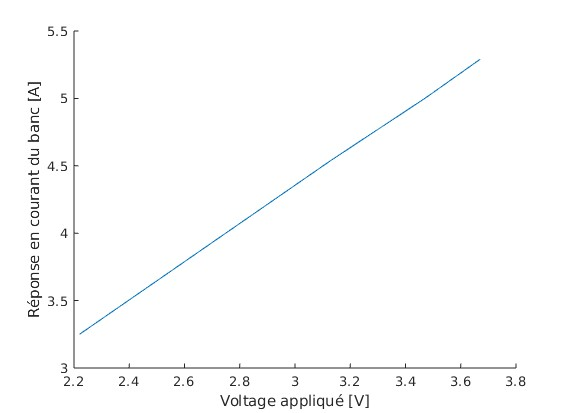
\includegraphics[width=0.5\linewidth]{IMAGES/ALEEL/voltagevscurant.jpg}
        \caption{Voltage appliqué vs réponse du banc de test.}
    \end{figure}
    Comme nous souhaitons appliquer $I_{a,nom}/2 = \frac{7.3}{2}=3.65A$ à la MCC, nous devons appliquer une commande de $5.1V$. \\
    
    \item Mesure de $T_{ea}$ et $T_r$ : \\
    La mesure est réalisée en envoyant un saut de tension à travers une source et un interrupteur, ce qui entraîne un saut de courant égal à la moitié du courant nominal de la machine à l'armature. Il est crucial de ne pas exciter la MCC afin d'éviter des perturbations et des oscillations indésirables, qui pourraient nuire à la qualité des mesures.
    \begin{figure}[hbt!]
        \centering
        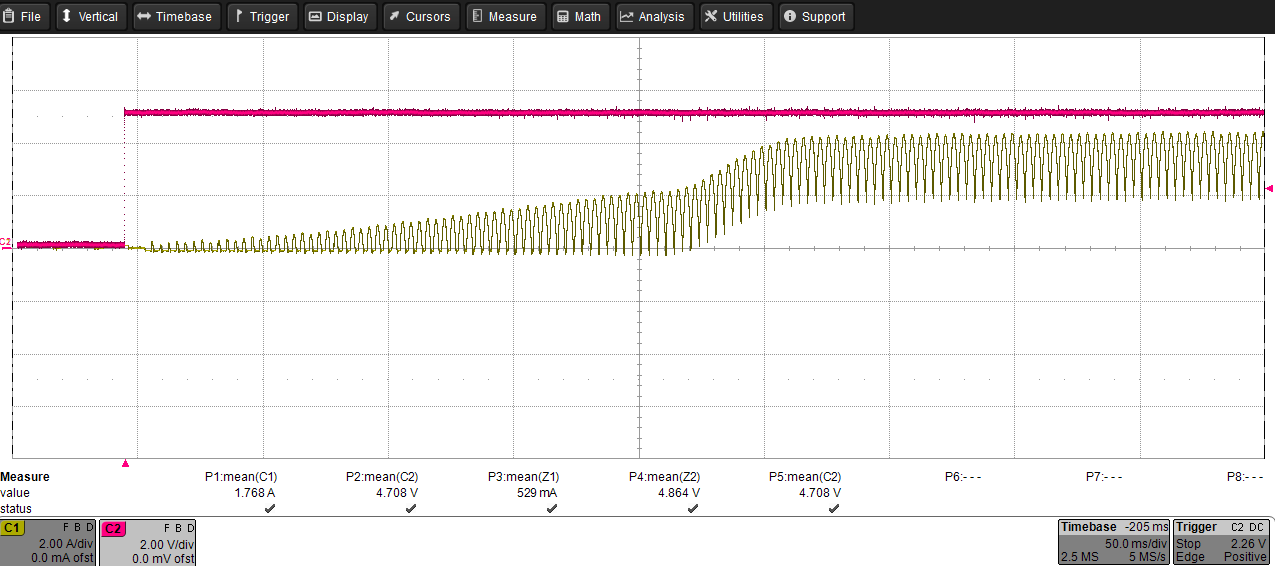
\includegraphics[width=0.7\linewidth]{IMAGES/ALEEL/LeCroy4.png}
        \caption{Capture de l'oscilloscope lors d'un essai de saut de commande de $0V$ à $5.1V$ pour une sortie de $3.65A$. La courbe rouge montre la commande de tension et la courbe verte, la réponse en courant.}
        \label{fig:sautCommande}
    \end{figure}
    
    D'après \ref{fig:sautCommande}, lors d'un saut de commande de $0V$ à $5.1V$, on peut mesurer le temps mort $T_r = 9.8 \pm 0.9ms$, qui correspond au délai initial du système avant que la sortie ne commence à réagir de manière significative au saut de tension appliqué. On peut également mesurer le temps de stabilisation, nécessaire au système pour atteindre une réponse stable après un saut de commande : $t_{ea} = \frac{t_a}{6} = 41.7 \pm 2ms$ (moyenne sur 6 tests).\\

    
    \item Mesure de $T_m$ :\\
    L'excitation est alimentée à ses valeurs nominales ($I_{ext} = 0.45A$), tandis que l'armature subit un saut de commande, via une source de tension et un interrupteur qui appliquent un step de $0$ à $5.1V$. Le rotor s'accélère et, une fois la vitesse nominale atteinte ($1500 \, \text{rpm}$), l'alimentation de l'armature par la source doit être coupée.

    \begin{figure}[hbt!]
        \centering
        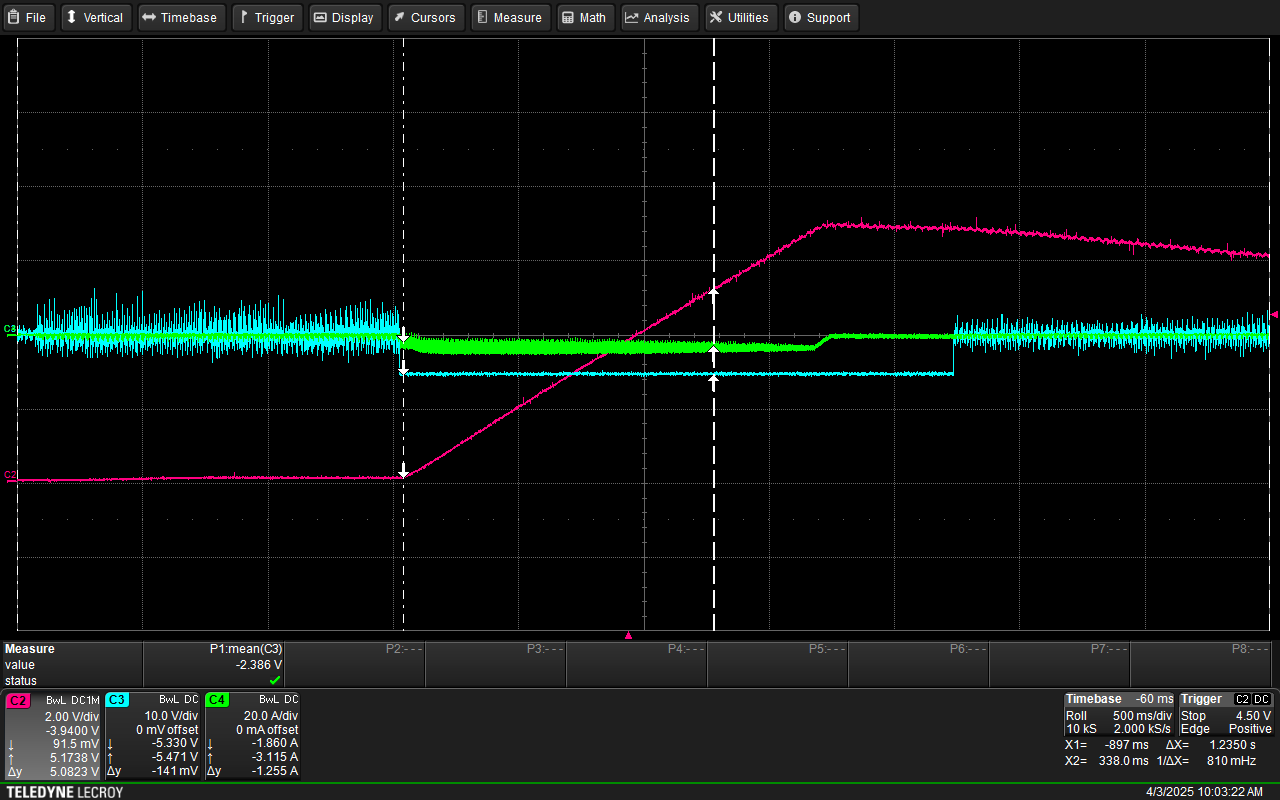
\includegraphics[width=0.7\linewidth]{IMAGES/ALEEL/LeCrtm2.png}
        \caption{Capture de l'oscilloscope lors d'un saut de commande de 0 à 5.1V avec excitation nominale. La courbe jaune représente la vitesse de l'arbre, la courbe bleue la commande en tension, et la courbe verte le courant d'armature.}
        \label{fig:testTm}
    \end{figure}
     
    Après avoir caractérisé l'équivalence tension/vitesse (\(294.8 \, \text{rpm/V}\)), nous pouvons mesurer le temps nécessaire à la MCC pour atteindre sa vitesse nominale (1500 rpm). Pour cela, nous observons le temps correspondant à une tension équivalente de $5.08V$. D'après \ref{fig:testTm}, nous obtenons $T_m = 1.21 \pm 0.02 \, s$ (moyenne sur 3 tests).\\

\end{itemize}

On peut maintenant calculé les valeur de coefficient du contrôleur après discrétisation en utilisant (2) et (4).
\begin{gather*}
    T_n = 4 T_{pE}=0.2079 \hspace{30pt} T_i = 8 \frac{T_{pE}^2}{T_1} = 8 \frac{T_{pE}^2}{T_M}=0.0178\\
    K_{cw1} = 0.9952 \hspace{30pt} K_{cw2} = 0.0048
\end{gather*}
Les coefficient de proportionnalité et intégrales après discrétisation se calculent: 
\[K_i=\frac{T_E}{T_i}=0.0563 \hspace{30pt} K_p=\frac{T_n-\frac{T_E}{2}}{T_i}=11.6758\\\]

%$T_n = 4 T_{pE} = 4(\frac{T_E}{2}+T_{ea} + T_r) = 0.2079$, $T_i = 8 \frac{T_{pE}^2}{T_m} = 0.0113$. Ainsi, après discrétisation : $K_p = \frac{T_n-T_E/2}{T_i} = 18.33$ et $K_i = \frac{T_E}{T_i} = 0.0884$. \\
%De même, pour le correcteur on obtient : $K_{cw1} = 0.9952$ et $K_{cw2} = 0.0048$.\\

\subsubsection{Essai Simulation}

\begin{figure}[hbt!]
    \centering
    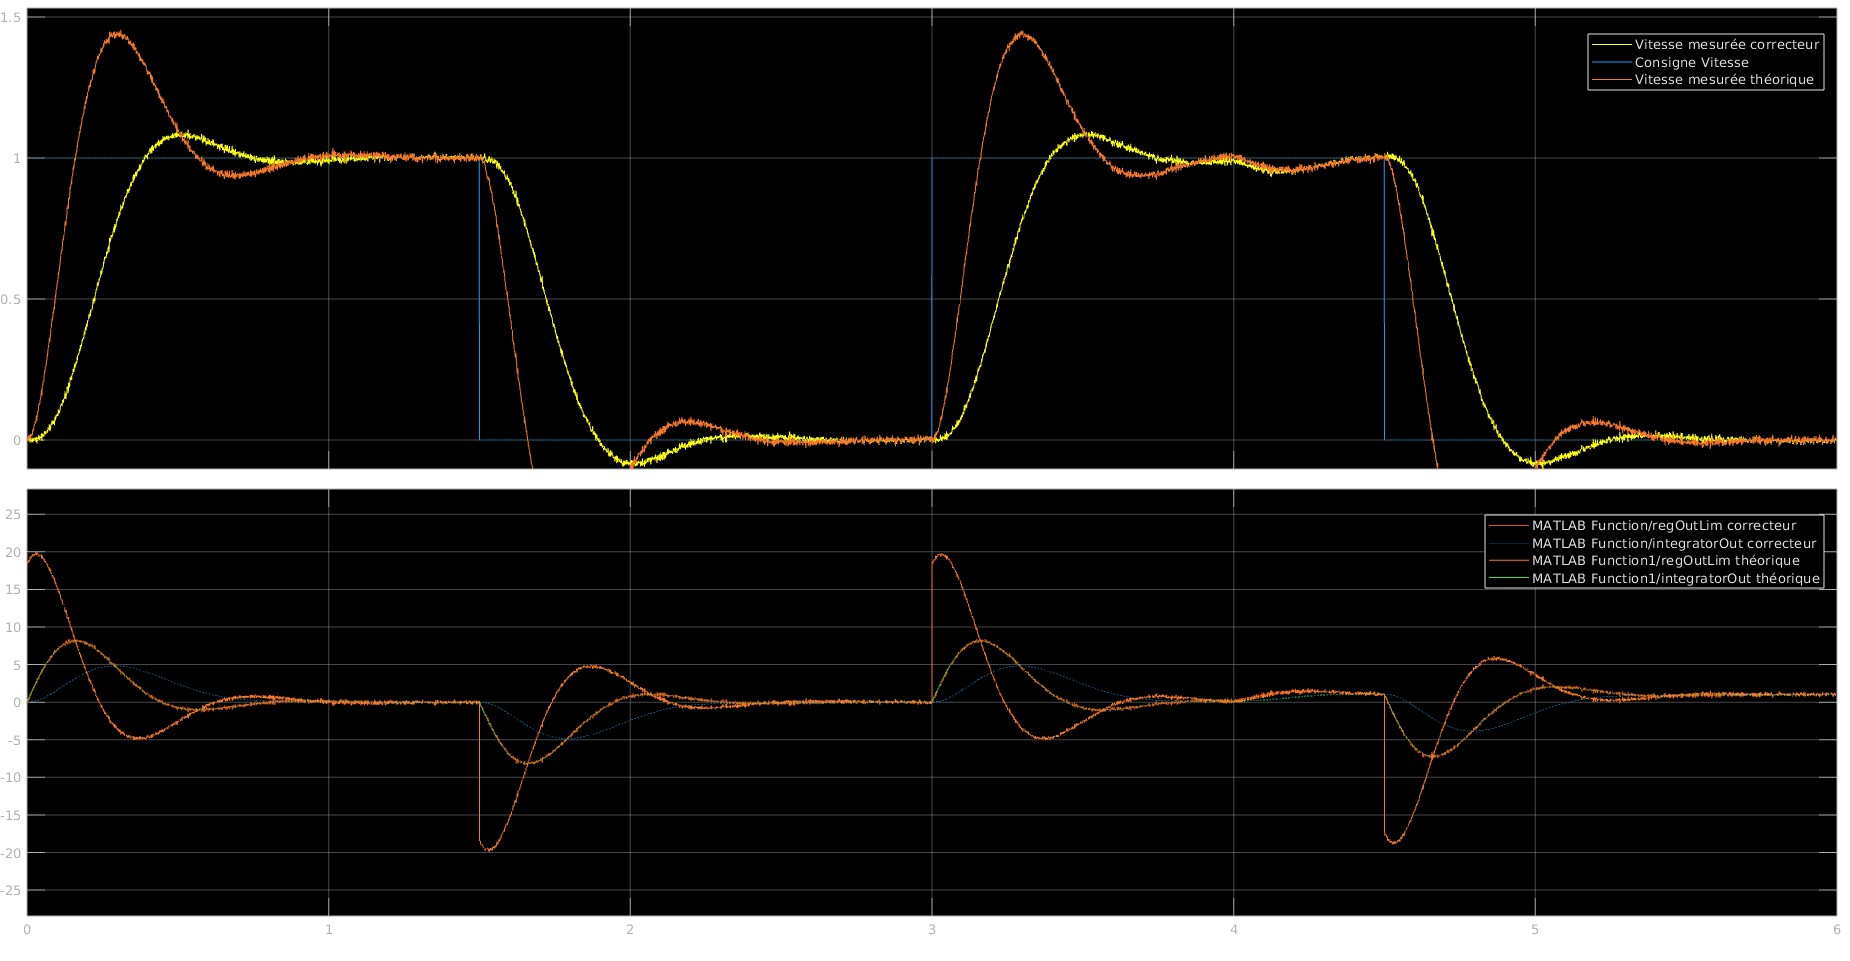
\includegraphics[width=\linewidth]{IMAGES/ALEEL/no_limitation.jpg}
    \caption{Simulink simulation du système sans limitation. Saut de charge à $m_r=1$ à $T=4s$.}
    \label{fig:noLimitations}
\end{figure}

\begin{figure}[hbt!]
    \centering
    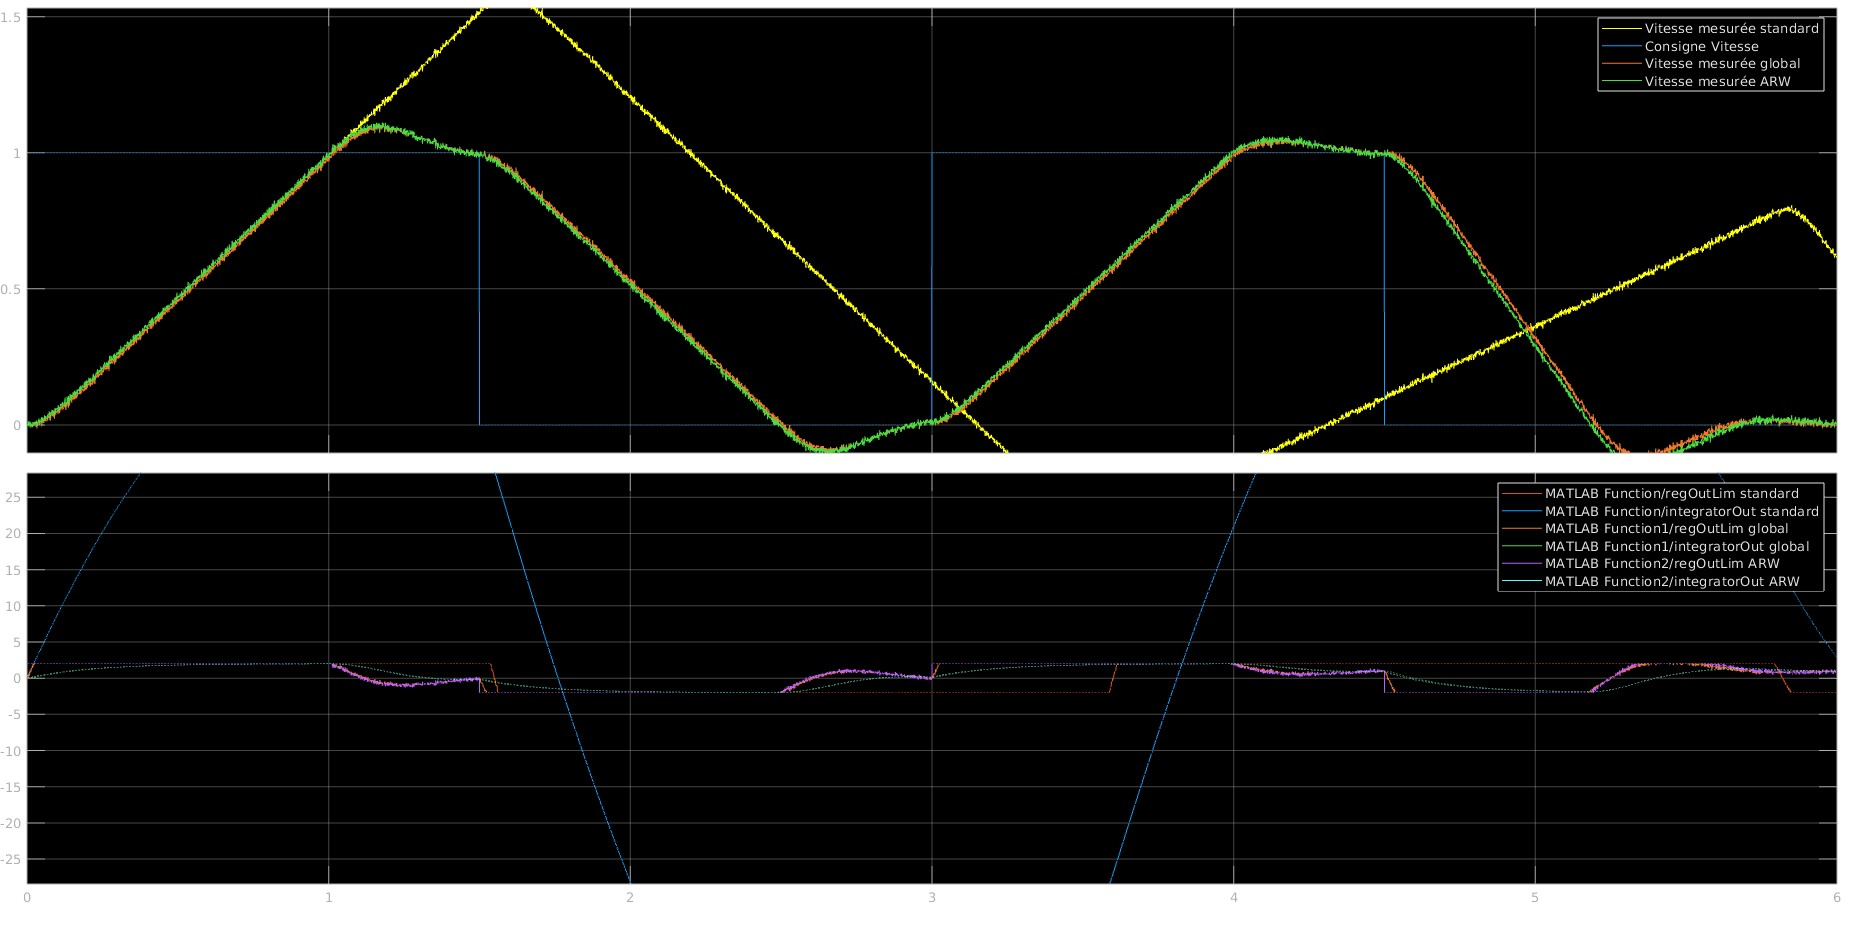
\includegraphics[width=\linewidth]{IMAGES/ALEEL/limitation.jpg}
    \caption{Simulink simulation du système sans limitation. Saut charge à $m_r=1$ à $T=4s$.}
    \label{fig:Limitations}
\end{figure}

D'après figure \ref{fig:noLimitations}, le système suit la consigne de vitesse sans limitation. Cependant, le modèle théorique présente un dépassement important de la vitesse, le correcteur permet ainsi de le limiter tout en gardant un temps de stabilisation égal.  \\
En comparant avec le système limité (\ref{fig:Limitations}), on remarque que le mode standard (sans correcteur ni ARW) ne peut pas être utilisé efficacement sur la MCC, car le dépassement est trop élevé et le système n'a pas le temps de se stabiliser autour de la consigne.  \\
Les deux autres modes (Global et ARW) réagissent de manière similaire: leur temps de stabilisation est plus long que dans les modes sans limitation, mais leur dépassement reste comparable à celui du mode avec correcteur seul.


\subsubsection{Test de l'installation réelle}
\paragraph{Mode Standard}
Sur la Figure \ref{fig:TestStandard}, on peut voir que lorsque le programme n'est equipé ni de correcteur, ni d'ARW mais seulement de la limitation, le vitesse va osciller autour de la vitesse de consigne en prenant beaucoup de temps pour l'atteindre. Pour une atteindre une vitesse nulle, le moteur va même passer par une vitesse négative en oscillant autour de la vitesse de consigne.
\begin{figure}[hbt!]
    \centering
    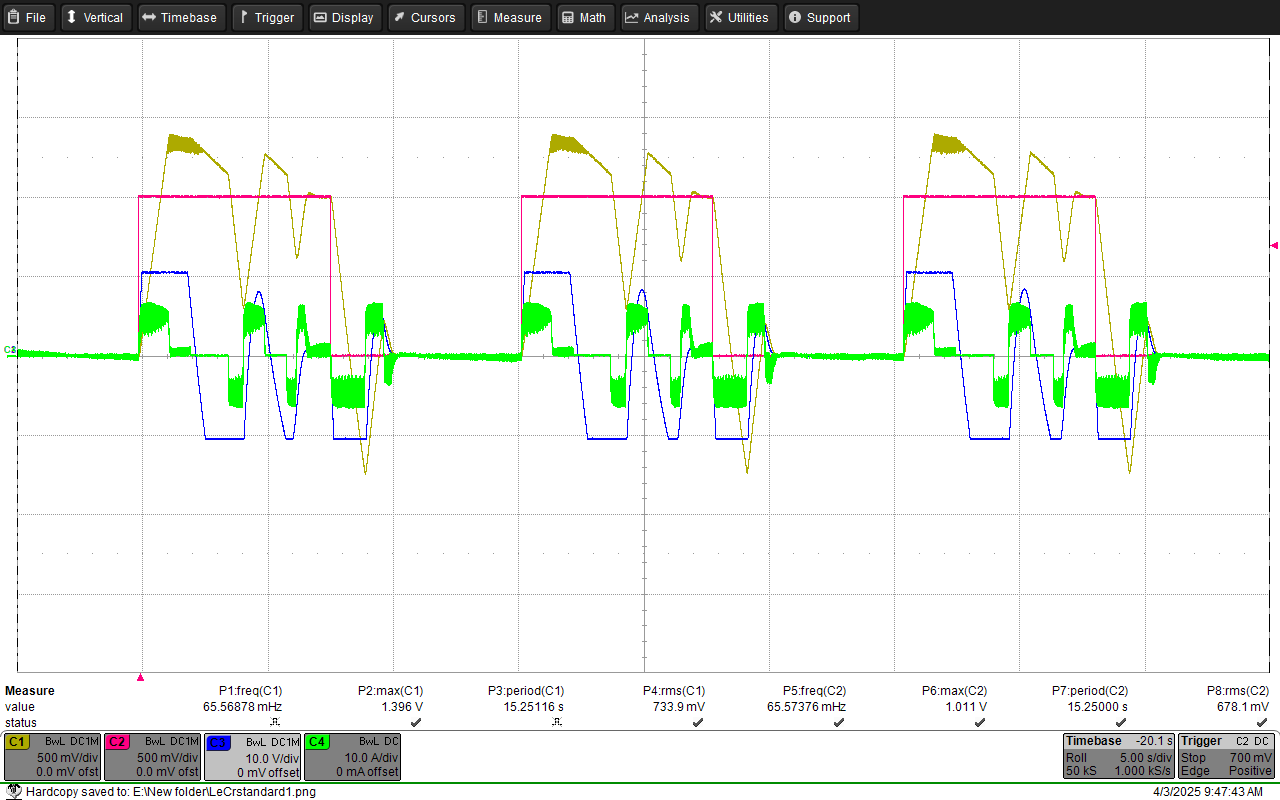
\includegraphics[width=\linewidth]{IMAGES/ALEEL/LeCrstandard2.png}
    \caption{Test de de l'installation réelle avec le mode Standard. La courbe jaune représente la vitesse réelle, la courbe rose la consigne de vitesse, la courbe bleu l'intégrateur et la courbe verte le courant dans l'armature de la MCC.}
    \label{fig:TestStandard}
\end{figure}

\paragraph{Mode Correcteur}
Le mode Correcteur ajoute un correcteur ce qui permet, comme le montre la Figure \ref{fig:TestCorrecteur}, de limiter l'overshoot.
\begin{figure}[hbt!]
    \centering
    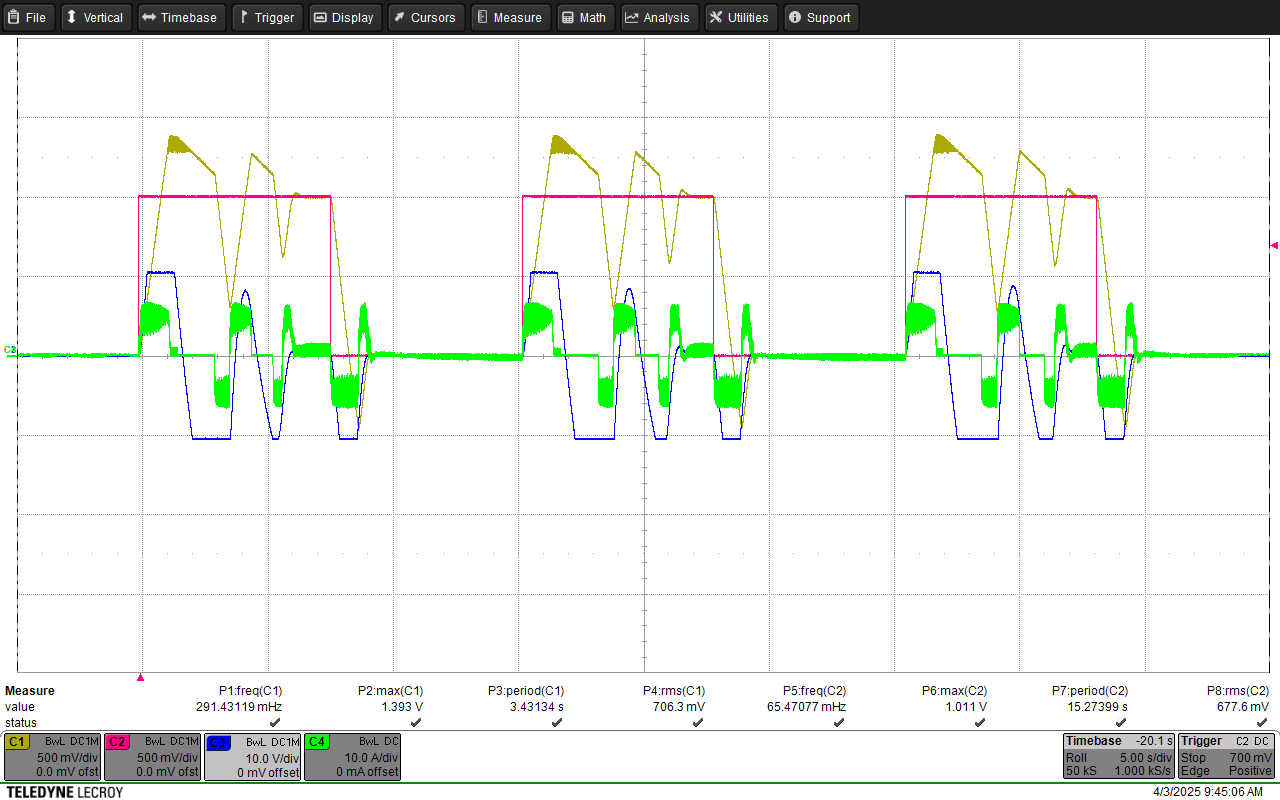
\includegraphics[width=\linewidth]{IMAGES/ALEEL/LeCrocorrector1.png}
    \caption{Test de de l'installation réelle avec le mode Correcteur. La courbe jaune représente la vitesse réelle, la courbe rose la consigne de vitesse, la courbe bleu l'intégrateur et la courbe verte le courant dans l'armature de la MCC.}
    \label{fig:TestCorrecteur}
\end{figure}

\paragraph{Mode ARW}
Le mode ARW ne possède pas de correcteur mais un anti-reset windup. Il limite l'accumulation de l'intégrateur, on le voit sur la Figure \ref{fig:TestARW}. La vitesse réelle se stabilise ainsi beaucoup plus vite et évite un trop gros dépassement de consigne et des oscillations autour de la vitesse de consigne.
\begin{figure}[hbt!]
    \centering
    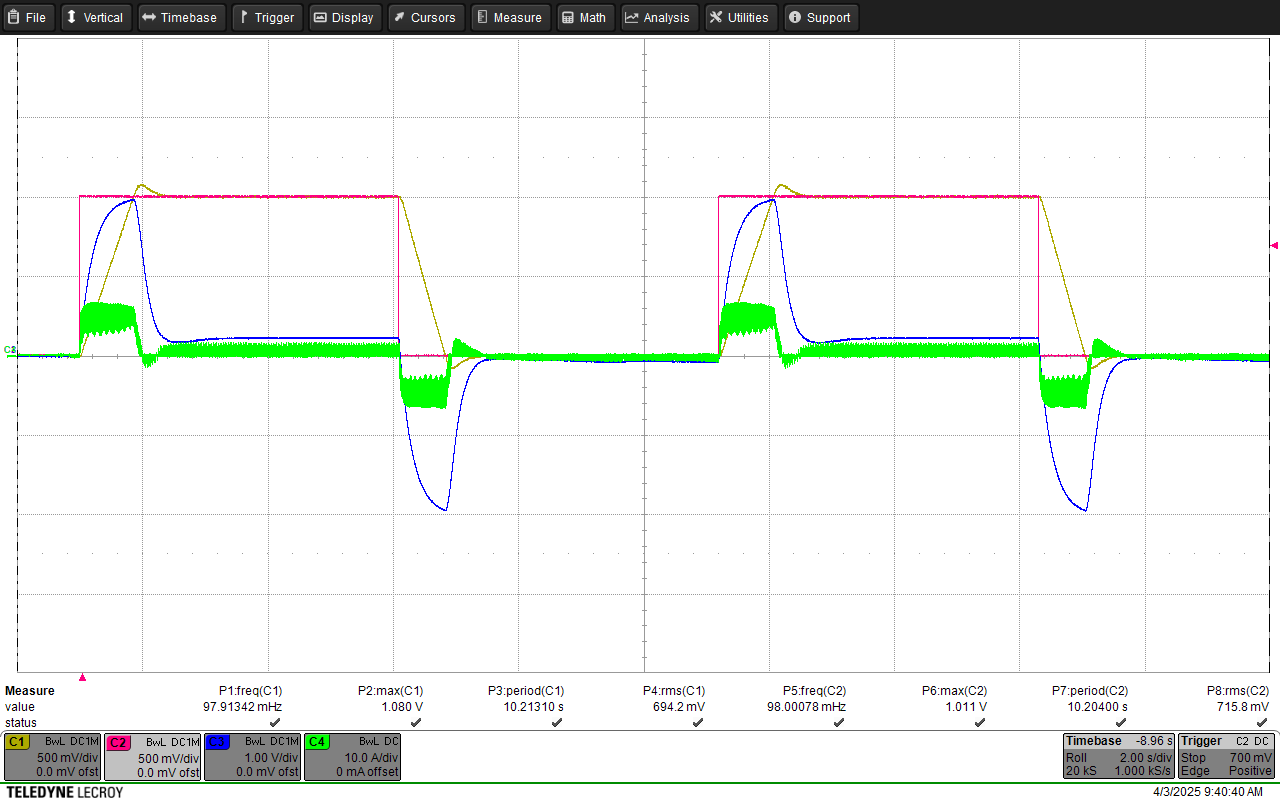
\includegraphics[width=\linewidth]{IMAGES/ALEEL/LeCroarw1.png}
    \caption{Test de de l'installation réelle avec le mode Anti-Reset Windup. La courbe jaune représente la vitesse réelle, la courbe rose la consigne de vitesse, la courbe bleu l'intégrateur et la courbe verte le courant dans l'armature de la MCC.}
    \label{fig:TestARW}
\end{figure}

\paragraph{Mode Global}
Le mode Global possède tout les éléments: la limitation, le correcteur et l'ARW. On voit ainsi que le contrôle se rapproche au mieux d'un cas idéal avec une réponse rapide, avec peu d'overshoot et sans oscillation autour de la valeur cible.
\begin{figure}[hbt!]
    \centering
    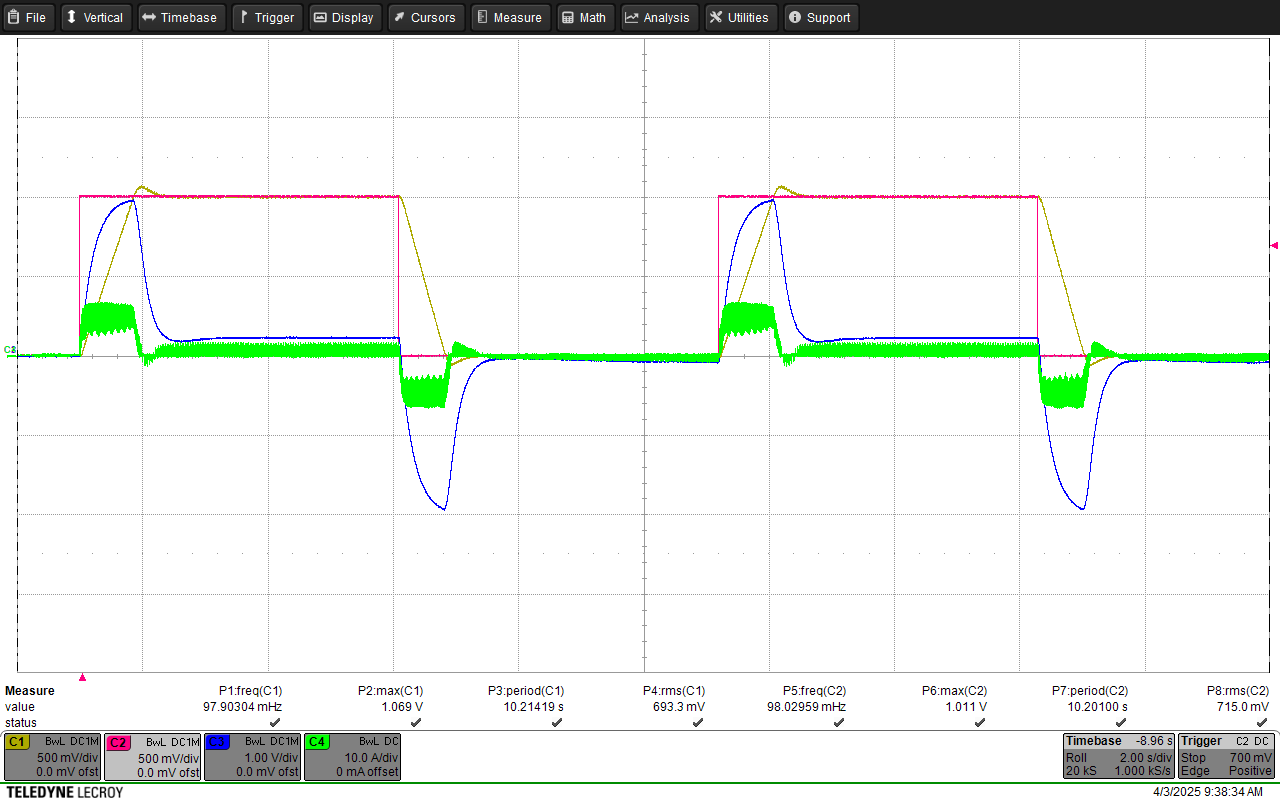
\includegraphics[width=\linewidth]{IMAGES/ALEEL/LeCroglobaly3.png}
    \caption{Test de de l'installation réelle avec le mode Global. La courbe jaune représente la vitesse réelle, la courbe rose la consigne de vitesse, la courbe bleu l'intégrateur et la courbe verte le courant dans l'armature de la MCC.}
    \label{fig:TestGlobal}
\end{figure}

\newpage
\subsection{Unitrol}
L'Unitrol permet un control de la tension générée par la MS. Il doit être relié au secteur avec soit : $300VAC$, soit $300V DC$. Nous avons choisi d'utiliser un pont de diode afin de transformer l'AC du réseau en DC. Un transformateur de tension doit également être utilisé afin de réduire la tension de ligne d'entrée.\\

Le schéma de cablage est le suivant : \begin{figure}[hbt!]
    \centering
    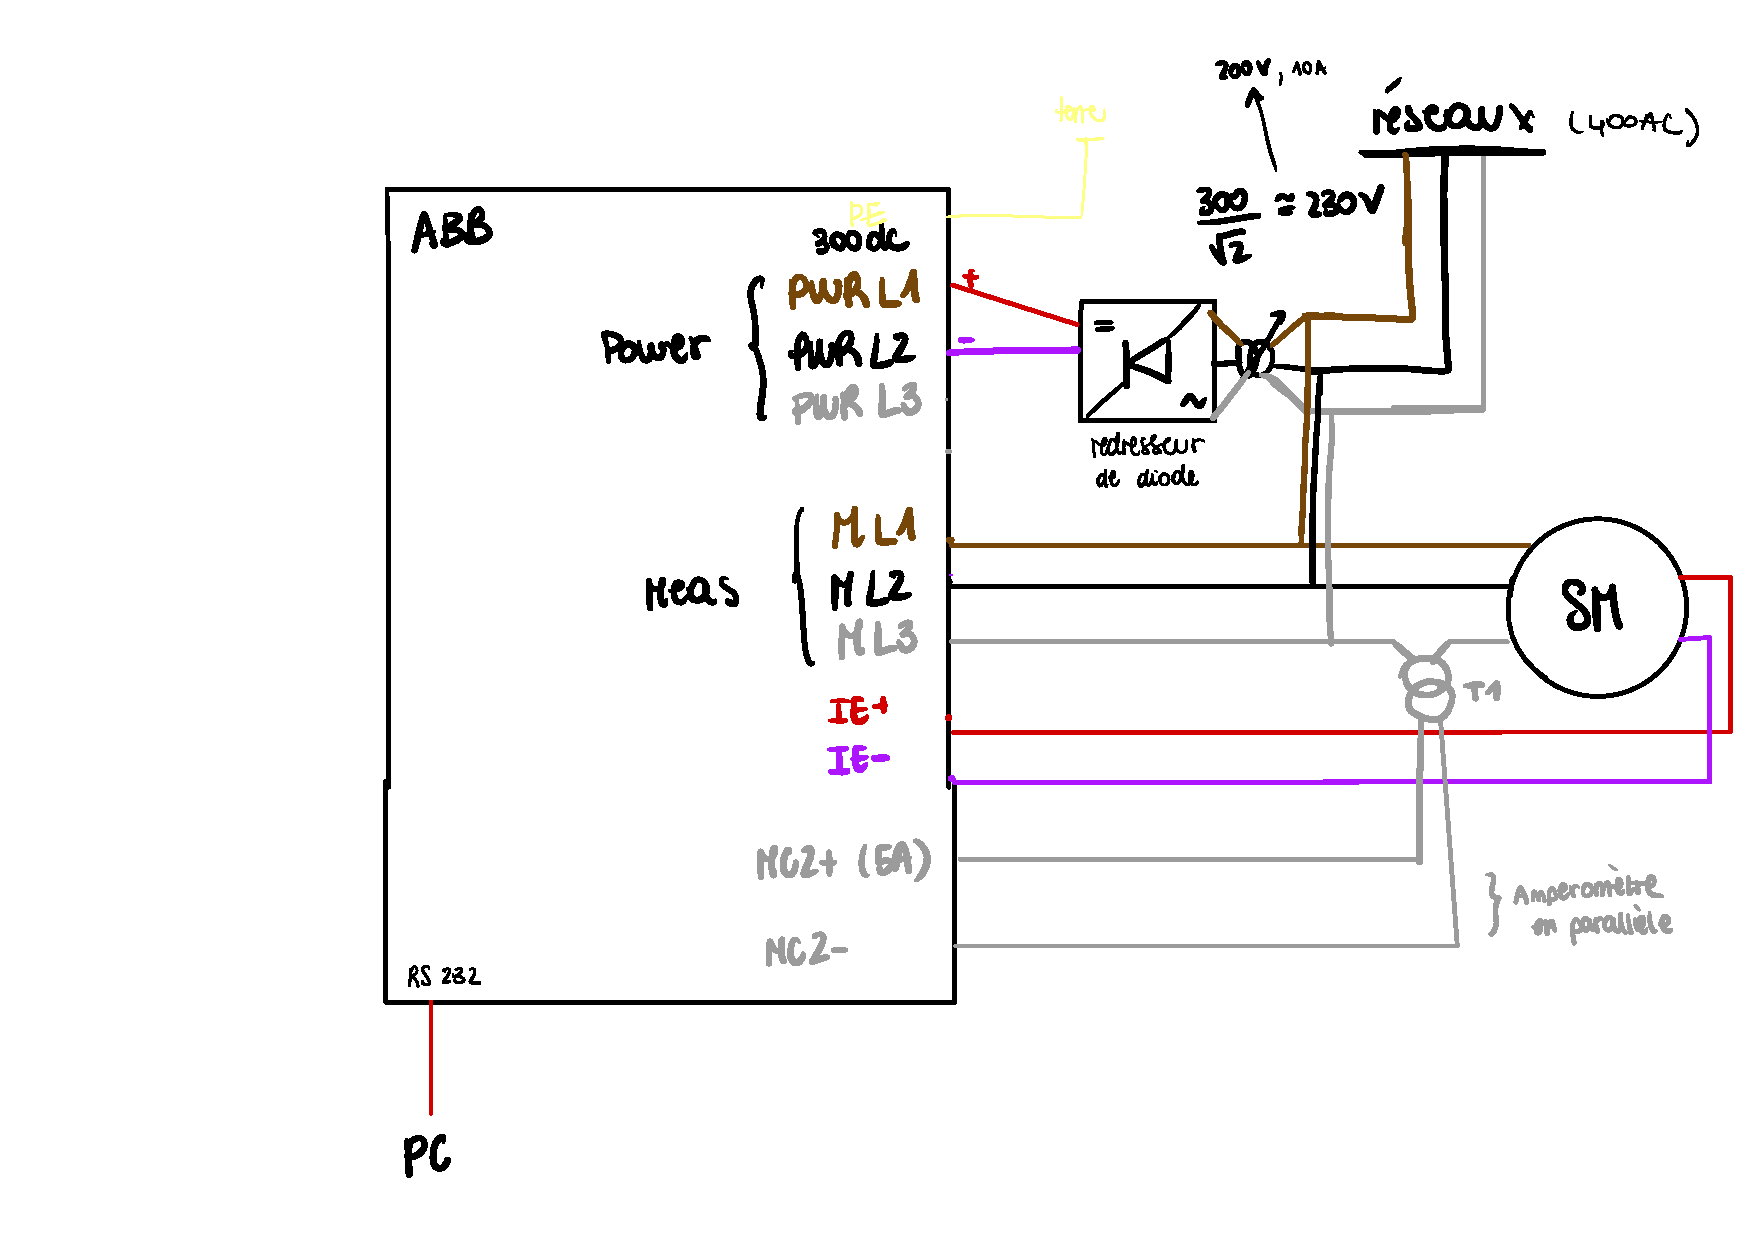
\includegraphics[width=0.8\linewidth]{IMAGES/ALEEL/Labo.pdf}

\end{figure}

Ce schéma peut être ainsi établi comme sur la figure \ref{fig:schema}. \\
\begin{figure}[hbt!]
    \centering
    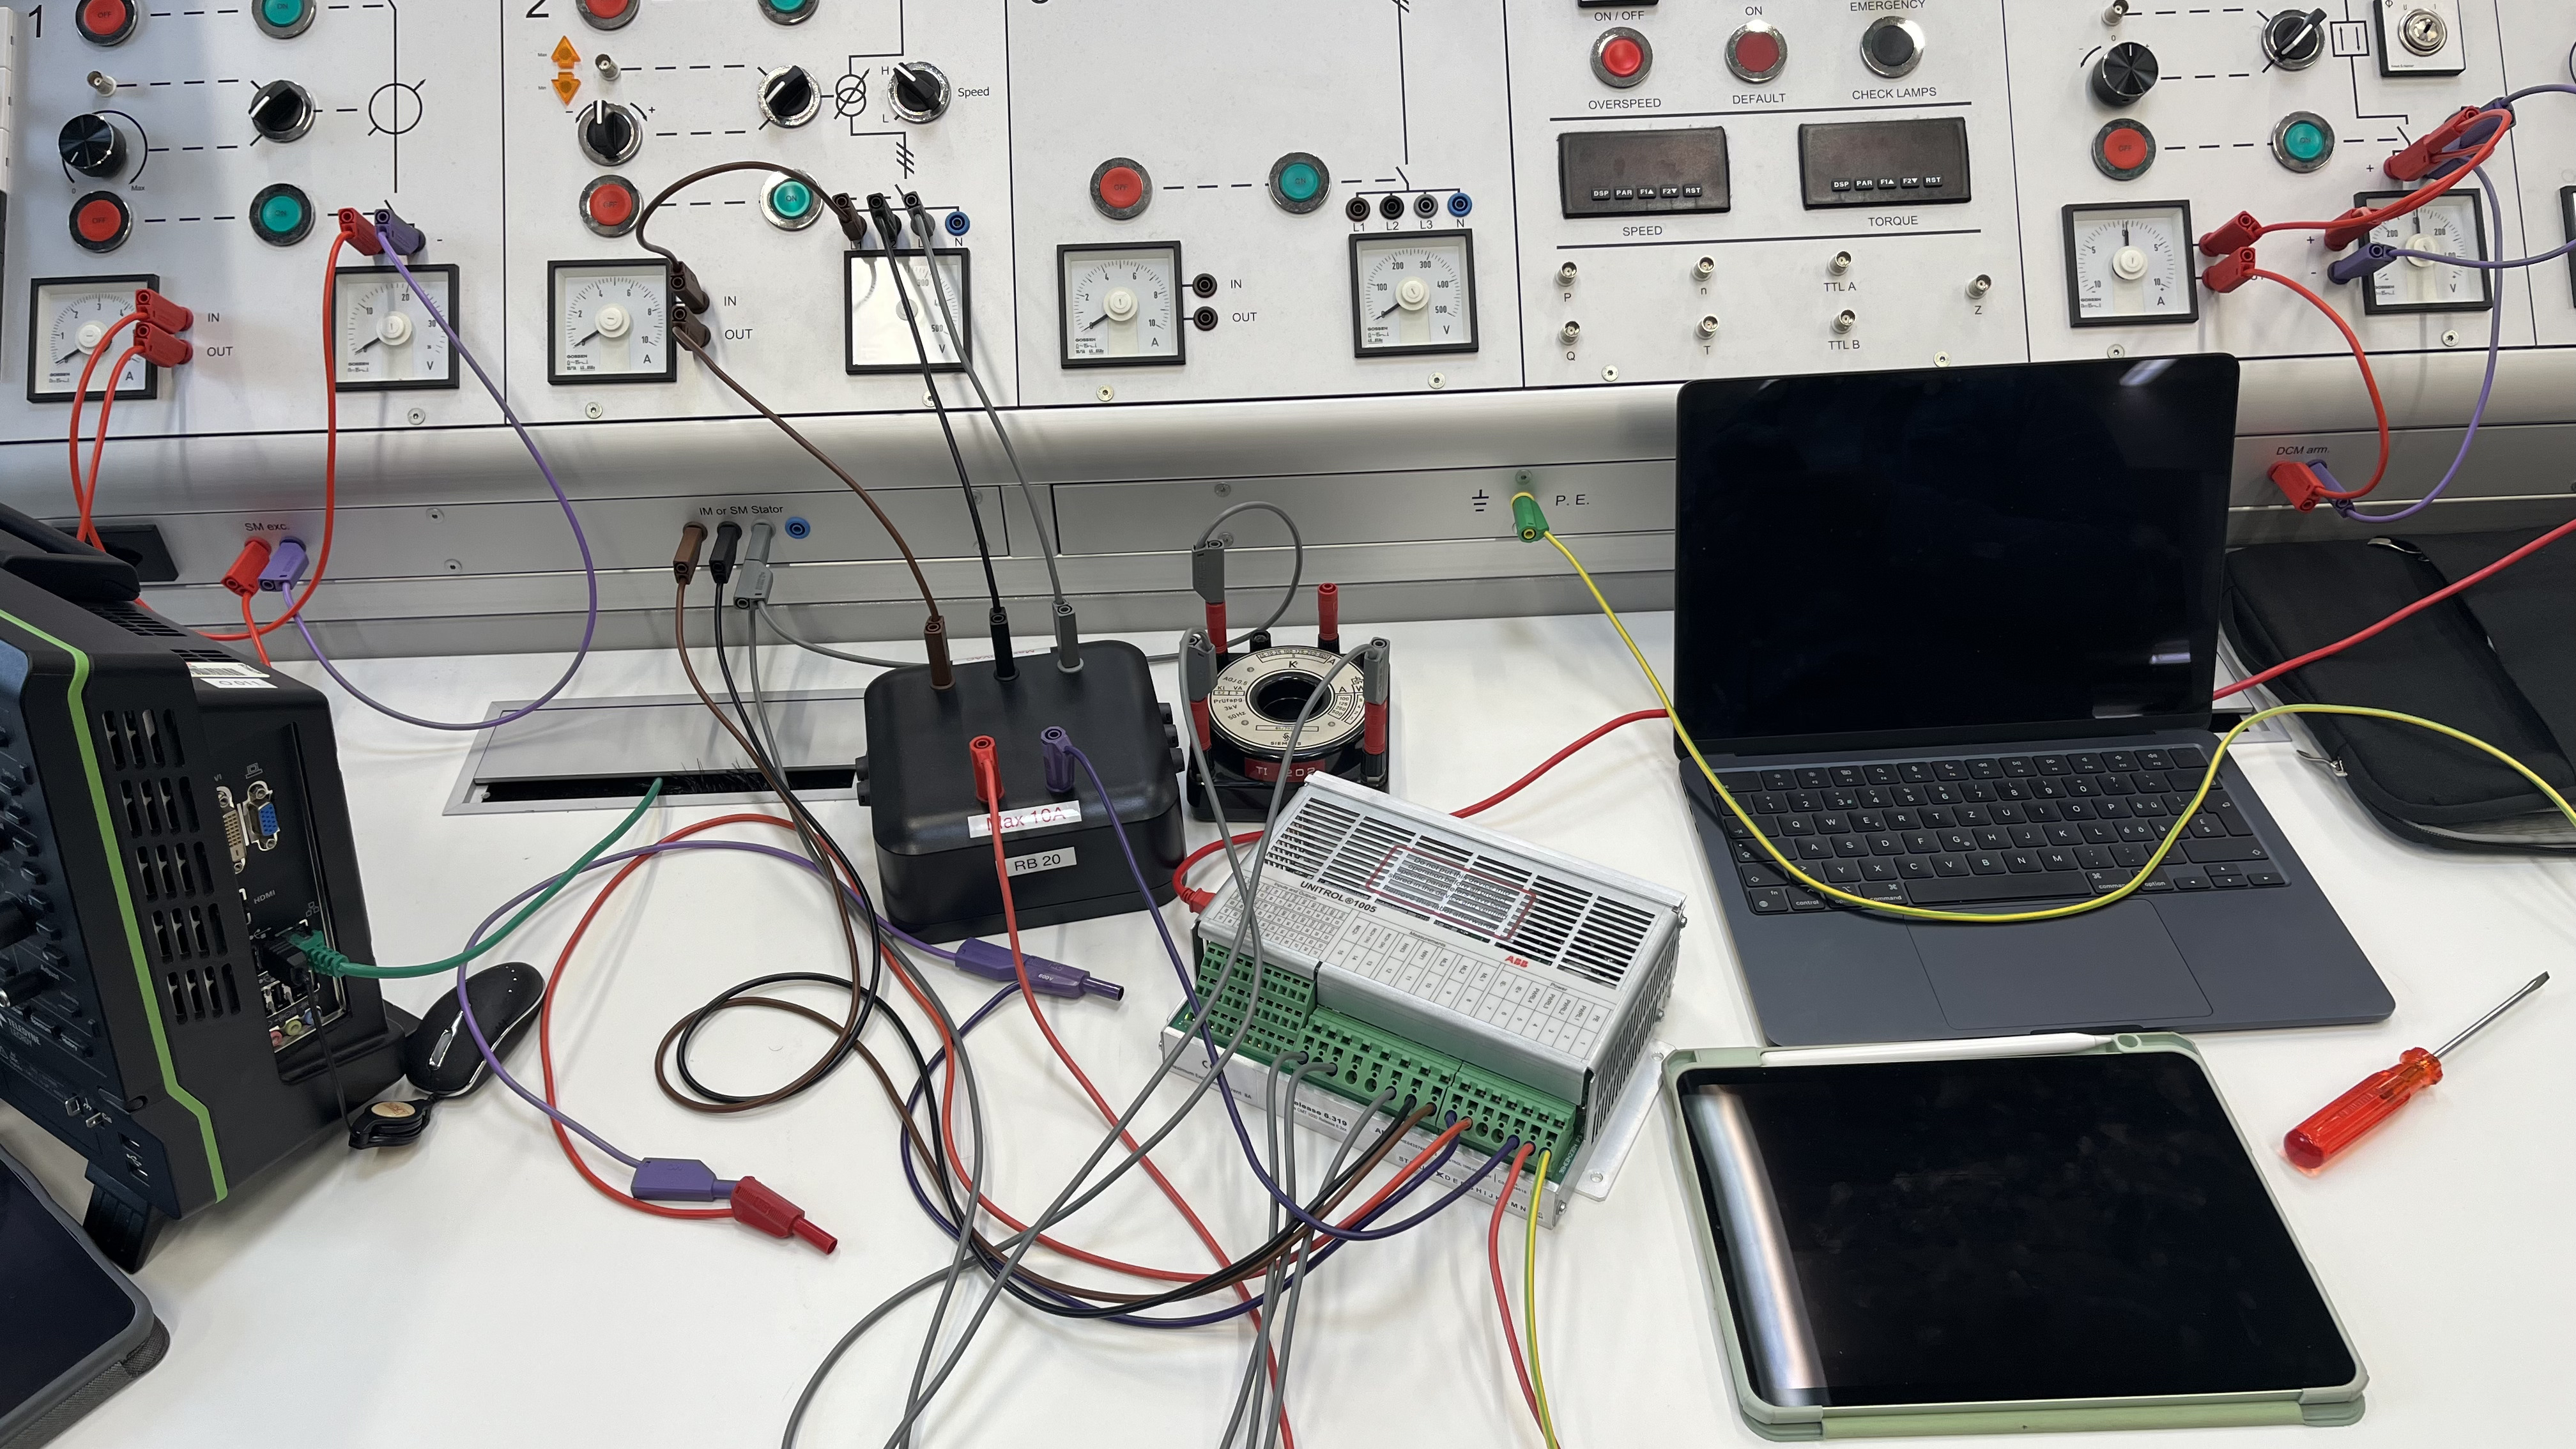
\includegraphics[width=0.8\linewidth]{IMAGES/ALEEL/IMG_2315.jpg}
    \label{fig:schema}
\end{figure}


Mode d'emploi : \begin{itemize}
    \item Connecter l'UNITROL à l'ordinateur via le cable USB. Onglet Communication : Port Configuration et choisir l'option USB. Bas à droite de l'onglet : choisir UNITROL 1005. Puis glisser flèche sur CONTROL
    \item Selon la figure \ref{fig:schema}, le courant d'excitation est activé lorsque l'interrupteur sur la pin 31 (Digital Input 5). Cette entrée doit être configurée sur l'UNITROL : \textbf{onglet Setup, Digital I/Os : DI5 Excitation ON} (pour une utilisation sans interrupteur, appuyer sur Normal inverse la polarité et active l'excitation). L'utilisation d'un interrupteur physique est conseillée car l'UNITROL se déconnecte régulièrement de l'ordinateur et il n'est plus possible de désactiver l'excitation. 
    \item Premièrement, il faut régler les paramètres de l'UNITROL :\textbf{ onglet Setup, System Data}. Ensuite : voir figure \ref{fig:systemData}.
    \begin{figure}[hbt!]
        \centering
        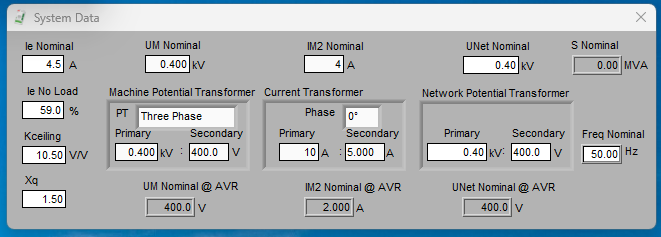
\includegraphics[width=0.5\linewidth]{IMAGES/ALEEL/systemData.png}
        \caption{Paramètres de l'UNITROL}
        \label{fig:systemData}
    \end{figure}
    
    \item Il faut ensuite calculer la valeur de $K_{ceiling} $ : correspond à l'inverse du PWM qu'il faut donner à l'excitation afin d'avoir la valeur nominale de tension de ligne lors d'un essai à vide. Selon le manuel de l'UNITROL, pour un contrôle optimal 5<$K_{ceiling}$<10. Nous avons alors : $PWM = 9.8$ soit $K_{ceiling} = 10.2$. 
    \item Tuning du PID : onglet : Tune, Auto pour avoir les paramètres du PID et Setpoint Adjust pour effectuer des sauts de commande en tensions. Le $V_P$ doit d'abord être choisi de telle sorte à éviter les oscillations. Ensuite le $T_i$ afin d'améliorer la vitesse du contrôleur puis le $T_b$. Nous avons trouvé les valeurs : $V_p = 10$, $T_i = 0.4s$ et $T_b = 0.01s$. Ces paramètres nous donnent lors d'un saut de commande de tension de $5\%$ une réponse du contrôleur suivant la figure \ref{fig:sautTension}.\begin{figure}[hbt!]
        \centering
        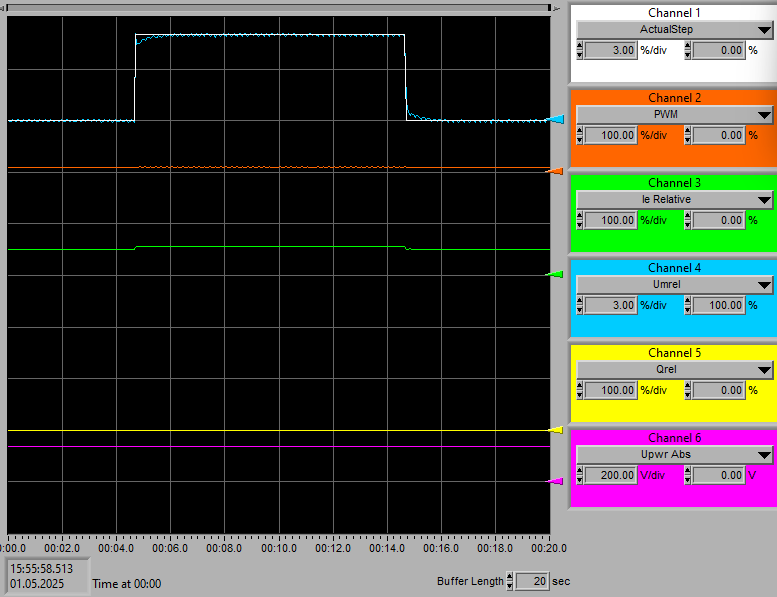
\includegraphics[width=0.5\linewidth]{IMAGES/ALEEL/step_close.png}
        \caption{Saut de commande de tension de $5\%$.}
        \label{fig:sautTension}
    \end{figure}
\end{itemize}

\warning Une fois effectué : ne pas oublier d'envoyer les paramètres dans l'UNITROL pour qu'ils restent même après déconnection : onglet File, Write Parameters to EEPROM.\\




\end{document}